% coding: UTF-8
%photonics.tex
% Fundamental of Photonics

\documentclass[UTF8]{ctexart}
%页眉
\usepackage{titleps,kantlipsum}
\newpagestyle{mypage}{
  \headrule 
  \sethead{\MakeUppercase{\thesubsection\quad \subsectiontitle}}{}{\thepage}
}
\settitlemarks{section,subsection,subsubsection}
\pagestyle{mypage}

%公式编号
\usepackage{mathtools}
\newtagform{mydefault}[\thesubsection-]{(}{)}
\usetagform{mydefault}
\makeatletter
\@addtoreset{equation}{subsection}
\makeatother

%插图
\usepackage{graphicx}
\usepackage{subfig}
\usepackage{float}

%颜色和color rectangle
\usepackage[dvipsnames]{xcolor}
\definecolor{ksc}{rgb}{0.24,0.36,0.65}
\definecolor{KSC}{named}{ksc}
\newcommand\crule[3][black]{\textcolor{#1}{\rule{#2}{#3}}}

%页面大小
\usepackage{geometry}
\geometry{a4paper,centering,scale=0.8}

%标题和日期
\title{\textcolor{ksc}{\textbf{\rightline{C H A P T E R}\\ \rightline{\Huge{11}}}}}
\date{}

%参考文献
\bibliographystyle{plain}

%目录
\renewcommand{\contentsname}{\textcolor{ksc}{统计光学}}
\renewcommand\thesection{\arabic{section}}
\renewcommand\thesubsection{\thesection.\arabic{subsection}}
\renewcommand\thesubsubsection{\Alph{subsubsection}.}
\renewcommand{\abstractname}{\null}
\setcounter{section}{11}

%图片和表格编号
\numberwithin{figure}{subsection}
\numberwithin{table}{subsection}
\renewcommand{\thefigure}{\thesubsection-\arabic{figure}}
\renewcommand{\thetable}{\thesubsection-\arabic{table}}

%微分算子优化和度定义
\usepackage{amsmath}
\DeclareMathOperator\dif{d\!}
\newcommand\degree{^\circ}

%行距
\usepackage{setspace}

%数学黑板粗体 P
\usepackage{amssymb}

%小黑色方块
\DeclareFontFamily{U}{MnSymbolC}{}
\DeclareFontShape{U}{MnSymbolC}{m}{n}{
  <-5.5> MnSymbolC5
  <5.5-6.5> MnSymbolC6
  <6.5-7.5> MnSymbolC7
  <7.5-8.5> MnSymbolC8
  <8.5-9.5> MnSymbolC9
  <9.5-11.5> MnSymbolC10
  <11.5-> MnSymbolCb12
}{}
\DeclareRobustCommand{\sqcdot}{%
  \mathbin{\text{\usefont{U}{MnSymbolC}{m}{n}\symbol{"69}}}%
}

%段落除首行缩进
\usepackage[notquote]{hanging}

\begin{document}
\nocite{*}
\maketitle
\noindent{\crule{\textwidth}{0.5cm}}
\tableofcontents

%摘要
\begin{abstract}
\begin{figure*}[h]
\centering
\subfloat[Max Born (1882-1970)]{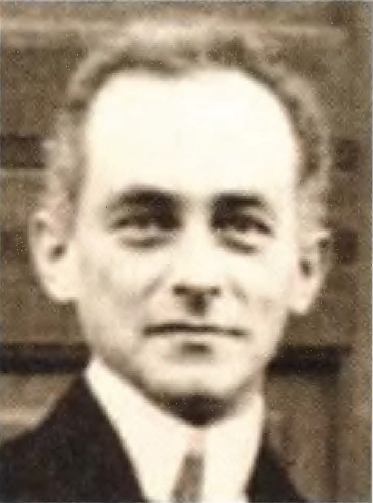
\includegraphics[width=0.2\textwidth]{maxborn.PNG}}
\hspace{.25in}
\subfloat[Emil Wolf (born 1922)]{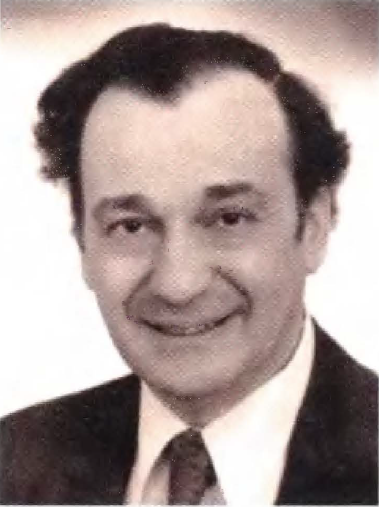
\includegraphics[width=0.2\textwidth]{emilwolf.PNG}}
\end{figure*}
这本由Max Born和Emil Wolf共同编写的《光学原理》首次于1959出版,着力于阐明光学中相干的重要性。Emil Wolf为光学相干理论的进步做出了重要贡献。
\end{abstract}

\newpage\textbf{统计光学}是对随机光的性质的研究。光的随机性,是由于光源和光传播经过的介质,均具有的、不可预测的扰动产生的。自然光(譬如说热源辐射的光)是随机的,因为它是极大量独立辐射、并具有不同频率和相位的原子的发射的光的叠加。光的随机性,也可能是光在,赋予了光波前随机扰动的粗糙表面、漫反射玻璃、湍急流体上散射的结果。对光的随机涨落的研究也称为\textbf{光的相干性理论}。
\par 我们在前面的章节中假设光是确定的或者“相干”的。一个相干光的例子是单色波\\$ u(r,t) = Re \{ U(r) \exp(j\omega t) \}$, 其中复振幅 $ U(r) $是确定的复函数,譬如说在球面波 [图11.0-1(a)]情况下$ U(r) = Aexp(-jkr)/r $,其波函数对时间和位置的依赖是完全周期的和可预测的。另一方面,对于随机光而言,波函数对于时间和位置的依赖 [图11.0-1(b)]不是完全可预测的,并且如果不借助统计学的方法,我们无法对其波函数进行一般性的描述。
\begin{figure}[H]
\centering
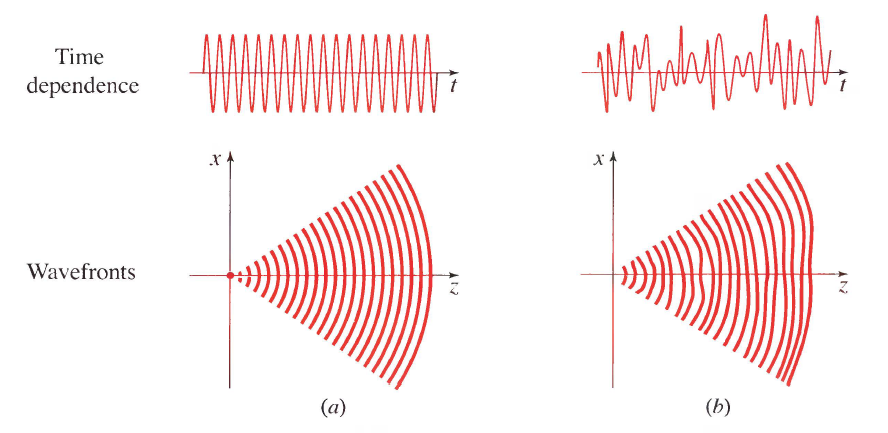
\includegraphics[width=0.9\textwidth]{11_0_1.PNG}
\caption{(a) 单色球面波(作为相干光的一个例子);
(b)随机光;的时间依赖性和波前。}
\label{fig: 11_0_1}
\end{figure}
\par 我们怎样,才能从随机光波的涨落中,提取出一些能描述这种涨落,并将此随机波与其它随机波区分开的有效的测度呢? 就比如说,三个波函数在某一位置随时间的变化,如图11.0-2所示的随机光波。显然,波(b)比波(a)更“密”,波(c)的包络比其余两波的包络涨落得“更快”。 
\begin{figure}[ht]
\centering
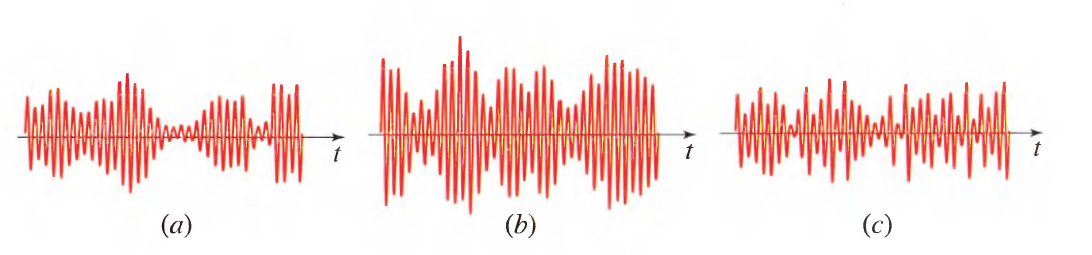
\includegraphics[width=0.9\textwidth]{11_0_2.PNG}
\caption{三个随机波的波函数的时间依赖性}
\label{fig: 11_0_2}
\end{figure}
\par 我们使用统计平均的概念,来描述大量非随机测量的特性,从而将这些随意的、定性的观察转化为定量的测度。因为随机函数$ u(r,t) $遵循特定定律(波动方程和边界条件),故其统计平均值一定也遵循特定的定律。光的相干性理论,利用制约这些统计平均值的定律和某些测度剖析了这些这些统计平均值的定义,我们根据这些测度将光分为\textbf{相干光}、\textbf{非相干光}、和更普遍的,\textbf{部分相干光}。
\bigbreak\noindent\textcolor{ksc}{\textbf{\textsl{本章}}}
\par 本章是对部分相干理论的一个介绍。我们若要充分理解光的相干性理论,必须熟悉随机场(关于空间和时间的多元随机函数)理论。然而,本章所论述的范围甚是有限,我们只需了解统计平均的概念便已足够。在 Sec. 11.1中,我们定义了两个描述随机光的统计平均值——光强和互相干函数,刻画了时间相干性和空间相干性,并建立了时间相干性和单色性之间的联系。 Sec. 11.1中部分相干光的例子证明,空间相干光不一定是时间相干的,单色光不一定是空间相干的。产生可见干涉条纹的能力是光的相干性的基本表现形式之一。Sec. 11.2专门讨论了随机光的相干定律。 Sec. 11.3的主题,是部分相干光在自由空间,和各种光学系统,包括成像系统中的传播。Sec. 11.4对随机光(部分偏振)的偏振理论做了简要的介绍。

\bigbreak\begingroup
\color{ksc}
\subsection{随机光的统计性质}
\endgroup
任意一光波均可用波函数$ u(r,t) = Re\{U(r,t)\} $来描述,其中,$ U(r,t) $为复波函数。譬如,对于单色光而言,$ U(r,t) $的形式为 $ U(r)\exp(j\omega t)$,对于多色光而言,$ U(r,t) $可能是多个不同$\nu$值的相似函数的累和(见Sec. 2.6A中对复波函数的讨论)。对于随机光而言,$ u(r,t) $ 和 $ U(r,t) $均为随机函数,我们用本节中引入的大量统计平均值,对其进行描述。

\bigbreak\begingroup
\color{ksc}
\subsubsection{光强}
\endgroup
相干(确定)光的光强$ I(r,t )$是复波函数$ U(r,t) $的绝对值的平方
\begin{equation}
I(r,t) = \lvert U(r,t) \rvert ^2 .
\end{equation}
(见 Sec. 2.2A 和 Sec. 2.6A)。对于单色确定光而言,这个强度是独立于时间的,但对于脉冲光而言,这个强度是随时间变化的。
\par 对于随机光而言, $ U(r,t) $是时间和位置的随机函数。因此,强度$ U(r,t) $也是随机的。我们定义\textbf{平均光强}为
\begin{equation}
I(r,t) = \langle \lvert U(r,t) \rvert ^2 \rangle .
\end{equation}
其中符号$ \langle \cdot \rangle $表示随机函数的各态历经的总体平均值。这意味着,我们在相同的条件下重复生成这个波,每次都得到一个不同波函数,并且该波在每个时间点和位置的平均强度是确定的。在没有歧义的情况下,我们简单地称$ I(r,t) $为光强(将 \textsl{平均}这个词隐去了)。  $ \lvert U(r,t) \rvert ^2 $这个量被称为\textbf{随机}或\textbf{瞬时光强}。对于确定光而言,由于每次生成的波函数都是相同的,故平均运算是多余的,(11.1-2)得到的值与(11.1-1)得到的值相等。
\par 如图 11.1-1(a) 和 (b) 分别所示,平均光强可能是时间独立的,亦可能是时间的函数。前者适用于光波是统计\textbf{平稳的}情况,即光波的统计平均值不随时间变化。瞬时光强随时间而随机涨落,但其统计平均值为常数。在这种情况下,我们用 $ I(r) $表示平均光强。平稳性并不代表常量性,平稳性代表的是平均值的常量性。由恒定电流加热的普通白炽灯发出的光,就是平稳随机光的一个例子,其平均强度 $ I(r) $是到灯的距离的函数,但不随时间变化。然而,如Fig.11.1-1(a)中所示,该光的随机强度 $ \lvert U(r,t) \rvert ^2 $却随位置和时间涨落。
\begin{figure}[ht]
\centering
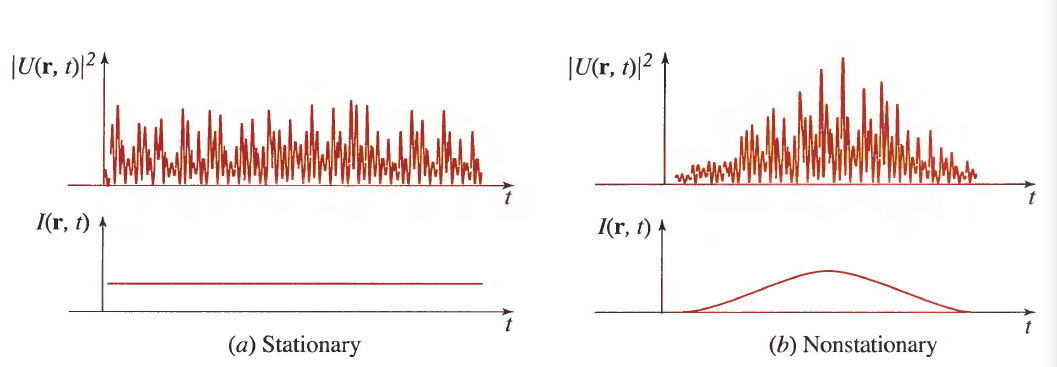
\includegraphics[width=0.9\textwidth]{11_1_1.PNG}
\caption{(a) 一个统计平稳波有一个不随时间变化的平均强度。(b) 一个统计非平稳波有一个随时间变化的平均强度。(a)中的点可以表示由恒定电流驱动的白炽灯发出的光,(b)中的点可以表示由脉冲电流驱动的白炽灯发出的光。}
\label{fig: 11_1_1}
\end{figure}
\par 当光是平稳的,(11.1-2)中的统计平均运算通常是在一个长时间段内求时间平均(而不是求各态平均),因此有
\begin{equation}
I(r) = \lim_{T\to\infty}\frac{1}{2T} \int_{-T}^T \lvert U(r,t) \rvert ^2 \dif t
\end{equation}

\bigbreak\begingroup
\color{ksc}
\subsubsection{时间相干性与频谱}
\endgroup
将\textsl{平稳}光在某一固定位置 $ r $处的涨落可看作是一时间的函数,则其平稳随机函数$ U(r,t) $有一常量光强$ I(r) = \langle \lvert U(r,t) \rvert \rangle ^2 $。出于简化,我们丢去光强对$ r $的依赖(因为$ r $是固定的),便有 $ U(r,t) = U(t) $ 和 $ I(r)=I $。
\par  我们用一个代表随机函数的“记忆”的时间尺度来描述$ U(t) $ 的随机涨落。时间间隔大于记忆时间的两个点的涨落是独立的,以致涨落过程“忘记”了它自己。在记忆时间内,函数$ U(t) $看起来是光滑的,但在大于记忆时间尺度的时间内测量时,函数$ U(t) $是“粗糙的”、“不稳定的”(见 图 11.0-2)。我们定义一个称为自相关函数的统计\textsl{平均}值,来建立对这种时间特性的定量测量。这个自相关函数描述了,波函数在给定时间延迟的两个瞬时,涨落的一致性,故其建立了构成波函数生成的基础的过程的时间尺度。
\bigbreak\noindent\textcolor{ksc}{\textbf{\textsl{时间相干函数}}}\\
作为一个时间延迟$ \tau $ 的函数,平稳复随机函数$ U(t)  $的自相关函数是$ U^\ast (t) $ 和 $ U(t+\tau) $乘积的平均值
\begin{equation}
G(\tau) = \langle U^\ast (t)U(t+\tau) \rangle
\end{equation}
或
\begin{equation}
G(\tau) = \lim_{T\to\infty}\frac{1}{2T} \int_{-T}^T U^\ast (t)U(t+\tau) \dif t
\end{equation}
(见 Sec. A.1 于 Appendix A).
\par 为了理解(11.1-4)中定义的重要性,思考一下复波函数的平均值$\langle U(t) \rangle = 0 $的情形。该情形成立于于相量$U(t)$的相位,如Fig. 11.1-2所示,在0 到 $ 2\pi $上等可能分布。乘积$ U^\ast (t)U(t+\tau) $的相位是相量$ U(t) $ 和相量 $ U(t+\tau) $之间的夹角,若$ U(t) $ 与 $ U(t+\tau) $是不相关的,则两相量之间的夹角在0 到 $ 2\pi $内随机变化,相量 $ U^\ast (t)U(t+\tau) $ 与实轴的夹角也因此是不确定的,即$ U^\ast (t)U(t+\tau) $等可能得取任意方向,这便使得其平均值——自相关函数$ G(\tau) $等于0。另一方面,若对于一给定的$\tau$,$ U(t) $ 与 $ U(t+\tau) $是相关的,则两相量之间便存在一定的关系,二者的涨落因而连接在一起,使得相量 $ U^\ast (t)U(t+\tau) $有一“偏爱”的方向,故其平均值$ G(\tau) $不为0。
\begin{figure}[ht]
\centering
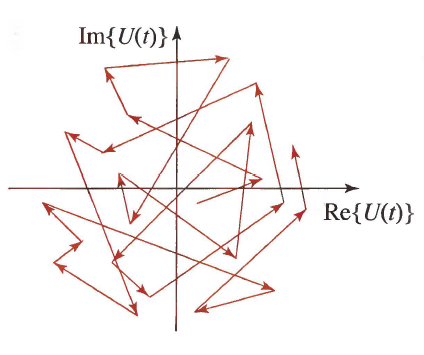
\includegraphics[width=0.4\textwidth]{11_1_2.PNG}
\caption{相量$ U(t) $的幅角在0 到 $ 2\pi $上均匀分布时$ U(t) $随时间的变化。其虚部和实部的平均值均为0,故$ \langle U(t) \rangle = 0 $。}
\label{fig: 11_1_2}
\end{figure}
\par 用光的相干性理论的话来说,自相关函数$ G(\tau) $称为\textbf{时间相干函数}。易知, $ G(\tau) $是 Hermitian 对称的,即 $ G(-\tau) = G^\ast (\tau) $, 并且 (11.1-2)定义的平均光强 $ I $ 等于$ G(\tau) $ 在 $ \tau =0 $处的取值,
\begin{equation}
I = G(0).
\end{equation}
\bigbreak\noindent\textcolor{ksc}{\textbf{\textsl{时间相干度}}}\\
时间相干函数$ G(\tau) $携带了平稳光的光强$ I = G(0) $和平稳光的相关(相干)度的信息。我们用归一化的自相关函数,给出了一对光强不敏感的相干性的测度
\begin{equation}
g(\tau) = \frac{G(\tau)}{G(0)} = \frac{\langle U^\ast (t)U(t+\tau) \rangle}{\langle U^\ast (t)U(t) \rangle},
\end{equation}
测度$g(\tau)$称为\textbf{复时间相干度},其绝对值不超过$1$
\begin{equation}
0\leq \lvert g(\tau) \rvert \leq 1
\end{equation}
\par $ \lvert g(\tau) \rvert $的值衡量了$ U(t) $ 与 $ U(t+\tau) $的相关度。若光是确定的且是单色的,譬如, $ U(t) =A \exp(j\omega_0 t) $,其中A是常数,计算(11.1-7)可得到
\begin{equation}
g(\tau) = \exp(j\omega_0 \tau),
\end{equation} 
此时,对于任意$ \tau $,均有$ g(\tau) = 1$,因而对于任意时间延迟$ \tau $,$ U(t) $ and $ U(t+\tau) $ 都是完全相关的。通常,随着$ \lvert\tau\rvert $增大,$ \lvert g(\tau) \rvert $从其最大值$ g(0) = 1 $处开始向两边衰减,只要$ \lvert\tau\rvert $足够大,两处的涨落变得不相关。
\bigbreak\noindent\textcolor{ksc}{\textbf{\textsl{相干时间}}}\\
若$\lvert g(\tau) \rvert $随时间延迟单调递减,则我们将$\lvert g(\tau) \rvert $降到某一规定值时 $ \tau_c $的值,作为对于涨落记忆时间的一个测度,$ \tau_c $称为\textbf{相干时间} (见 图 11.1-3)。
\begin{figure}[H]
\centering
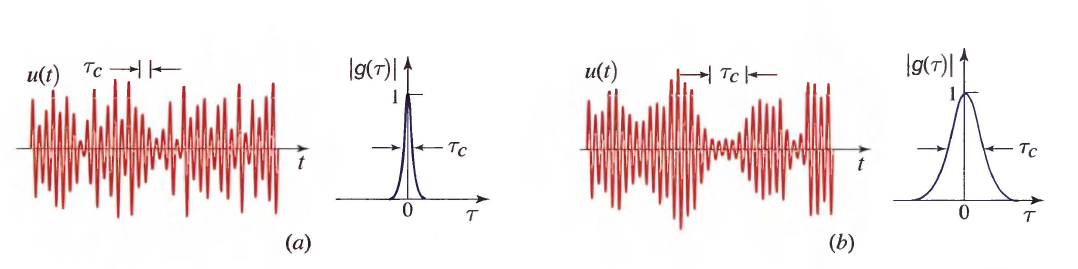
\includegraphics[width=0.9\textwidth]{11_1_3.PNG}
\caption{具有(a)短相干时间、 (b)长相干时间的光场的波函数、复时间相干度的模$\lvert g(\tau) \rvert $、相干时间$ \tau_c$的说明性示例。波函数的振幅和相位,以近似等于相干时间的时间常数随机变化。在两个情形下,相干时间$ \tau_c $均比一个光周期的持续时间要长。在相干时间内,波是相当可预测的,且可近似为一个正弦曲线。然而,即使知道波在某一特定时刻的振幅和相位,我们也无法预测波在距离该时刻相干时间外的振幅和相位。}
\label{fig: 11_1_3}
\end{figure}
\par  $\tau < \tau_c $时,涨落是“强'”相关的,$ \tau > \tau_c $时,涨落是弱相关的。一般来说, $ \tau_c $是函数$\lvert g(\tau) \rvert $的宽度。虽然对一个函数宽度的定义相当随意 (见 Sec. A.2 于 Appendix A),但是我们一般用功率等价宽度
\begin{equation}
\tau_c = \int_{-\infty}^{+\infty} \lvert g(\tau) \rvert ^2 \dif \tau
\end{equation}
作为相干时间的定义[见 (A.2-8) 并注意 $ g(0) = 1$]. 对于单色光而言,在每一处均有$\lvert g(\tau) \rvert = 1$,故其相干时间为无穷大。
\bigbreak\noindent{\crule[ksc]{\textwidth}{0.2cm}}
\textbf{EXERCISE 11.1-1} \\
\textbf{相干时间.} 证明下面复时间相干度的定义与(11.1-10)中$ \tau_c $的定义一致:
\begin{equation}
g(\tau) = 
\begin{cases}
\exp(-\frac{\lvert \tau \rvert}{\tau_c}) & (exponential) \\
\exp(-\frac{\pi \tau^2}{2\tau_c^2}) & (Gaussian)
\end{cases}
\end{equation}
在每个情况下,当$ \tau $从0增大到$ \tau_c $时,$ \lvert g(\tau) \rvert $衰减为原来的多少?\\
\noindent{\crule[ksc]{\textwidth}{0.2cm}}
\par 若研究的光学系统中所遇到的时间延迟差,均远小于光的相干时间$ \tau_c $,则我们可认为光是几乎完全相干的。也就是说,若研究的光学系统中所遇到光程差,均远小于距离$c\tau_c$,则我们可认为光是几乎完全相干的。因此,距离
\begin{equation}
l_c = c\tau_c
\end{equation}
也称为 \textbf{相干长度}。
\bigbreak\noindent\textcolor{ksc}{\textbf{\textsl{功率频谱密度}}}\\
为了确定随机光的\textsl{平均}频谱,我们对随机函数 $ U(t) $做一次傅里叶分解。频率为$ \nu $的成分的振幅就是傅里叶变换(见 Appendix A)
\begin{equation}
V(\nu) = \int_{-\infty}^{+\infty} U(t) \exp(-j2 \pi \nu t) \dif t .
\end{equation}
频率在区间$ \nu $ 到$ \nu +\dif \nu $ 之间的成分在单位面积内的平均能量为$ \langle \lvert V(\nu) \rvert ^2 \rangle \dif \nu $,故 $ \langle \lvert V(\nu) \rvert ^2 \rangle $代表了光的频谱能量密度(单位面积内的能量)。注意,复波函数$ U(t) $被定义为波函数$u(t)$对应的相量(见Sec. 2.6A),故对于负的 $ \nu $,$ V(\nu) = 0 $。
\par 因为一个真正平稳的函数 $ U(t) $是无限延伸的并且携带无穷的能量,所以我们考虑函数$ U(t) $的频谱\textsl{功率}密度而不是考虑 $ U(t) $的频谱能量密度。我们先对函数$ U(t) $在宽度为T的窗口内进行截断傅里叶变换
\begin{equation}
V_T (\nu) = \int_{-T/2}^{+T/2} U(t) \exp(-j2 \pi \nu t) \dif t
\end{equation}
则$ \langle \lvert V_T (\nu) \rvert ^2 \rangle $即为$ U(t) $在窗口内的频谱能量密度,所要的功率频谱密度是单位时间内的能量$ (1/T) \langle \lvert V_T (\nu) \rvert ^2 \rangle $。我们取极限$ T \to \infty $将时间窗口延伸至无穷,便得到
\begin{equation}
S(\nu) = \lim_{T \to \infty} \frac{1}{T} \langle \lvert V_T (\nu) \rvert ^2 \rangle ,
\end{equation}
$S(\nu)$称为\textbf{功率频谱密度},其只在非负频率处有非0值。因为复波函数$ U(t) $被定义为波函数$u(t)$对应的相量,故$ \lvert U(t) \rvert ^2$代表单位面积上的功率,或者说代表光强($ W/cm^2 $),$ S(\nu) \dif \nu $代表频率在区间$ \nu $ 到$ \nu +\dif \nu $ 之间的成分在单位面积上的平均功率,所以说$ S(\nu) $代表的是\textbf{频谱强度密度}。$ S(\nu) $经常被简称为\textbf{频谱密度}或\textbf{频谱}。所有频谱的平均强度的总和为积分
\begin{equation}
I = \int_0^\infty S(\nu) \dif \nu .
\end{equation}
\par 由(11.1-4)定义的自相关函数 $ G(\tau) $与由(11.1-15)定义的频谱密度 $ S(\nu) $可被证明是一组傅里叶对 (见 Prob. 11.1-5),
\begin{equation}
S(\nu) = \int_{-\infty}^{+\infty} G(\tau) \exp(-j2 \pi \nu \tau) \dif \tau .
\end{equation}
此关系式称为 \textbf{Wiener-Khinchin 定理}。\\
\par 代表一个彩色图像(例如 图 11.1-4)的光波有随位置 $ r $变化的频谱,图中显示的每一个谱轮廓都对应一个可感知的颜色。
\begin{figure}[ht]
\centering
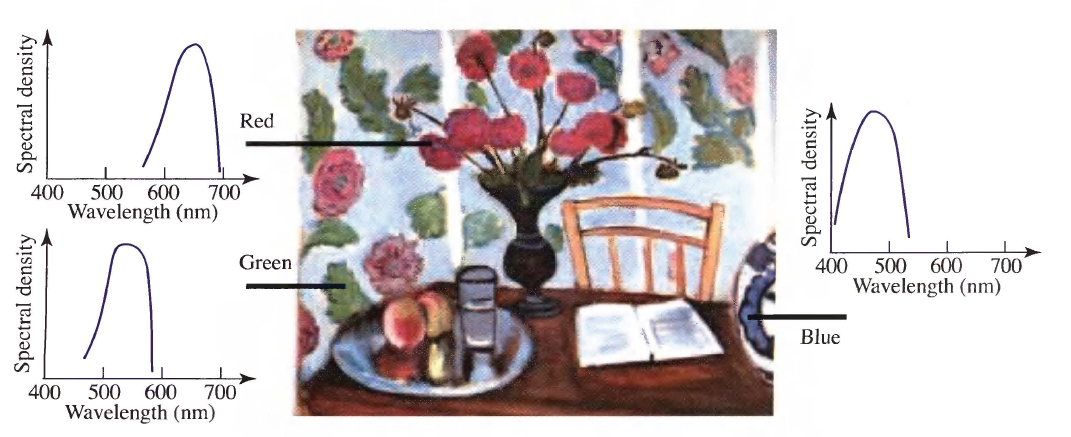
\includegraphics[width=0.9\textwidth]{11_1_4.PNG}
\caption{ 在一个彩色图像(Dahlias,Henri Matisse)中的三个位置处,以波长作为自变量的频谱密度函数的变化。}
\label{fig: 11_1_4}
\end{figure}
\bigbreak\noindent\textcolor{ksc}{\textbf{\textsl{频谱宽度}}}\\
光的频谱通常限制于一中心频率为$ \nu_0 $的窄带。光的\textbf{频谱宽度}, 或 \textbf{线宽}指的是频谱密度 $ S(\nu) $的宽度$ \Delta \nu $。由于 $ S(\nu) $ 与 $ G(\tau) $之间的傅里叶变换关系,二者的宽度是负相关的,即宽频谱的光源的相干时间短,窄线宽的光源相干时间长( 如 图 11.1-5 所示)。在单色光的极限情况下,$ G(\tau) = I \exp(j\omega_0 \tau) $,故相应的频谱强度密度$ S(\nu) = I \delta (\nu - \nu_0) $只包含单一的频率成分$ \nu_0 $。此时,$ \tau_c = \infty $ ,$ \Delta \nu = 0$。我们可以使用光滤波片缩小光源的频谱宽度来增加光源的相干时间,如此获得的相干性是以损失光能为代价的。
\begin{figure}[H]
\centering
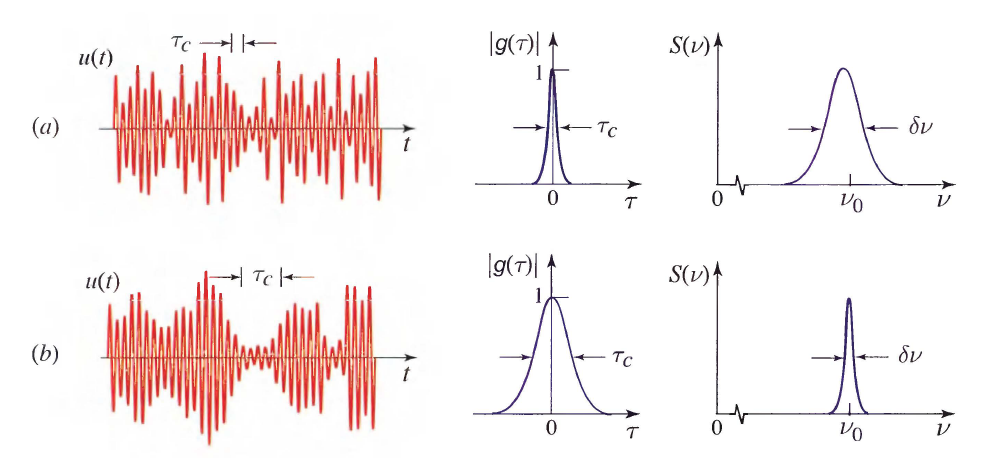
\includegraphics[width=0.9\textwidth]{11_1_5.PNG}
\caption{两个随机波的波函数、复时间相干度的模、频谱密度。}
\label{fig: 11_1_5}
\end{figure}
\par 有多种对频谱宽度的定义,最常见的定义为函数$ S(\nu) $的半峰全宽(full width of half maximum, FWHM)。如表 11.1-1所示(亦可见 Appendix A, Sec. A.2),相干时间与频谱宽度的精确关系依赖于频谱的轮廓。\\
\begin{table}
\caption{相干时间与频谱宽度的精确关系}
\begin{center}
\begin{tabular}{lccc}
\hline
频谱密度 & Reactangular & Lorentzian & Gaussian \\
\hline
频谱宽度 $ \delta \nu_{FWHM} $ & $ \frac{1}{\tau_c} $ & $ \frac{1}{\pi \tau_c} \approx \frac{0.32}{\tau_c} $ & $ \frac{\sqrt{2 ln2 / \pi}}{\tau_c} \approx \frac{0.66}{\tau_c} $ \\
\hline
\end{tabular}
\end{center}
\end{table}
\par 另一种对频谱宽度的合理定义为
\begin{equation}
\Delta \nu_c = \frac{(\int_0^\infty S(\nu) \dif \nu)^2}{\int_0^\infty S^2(\nu) \dif \nu}.
\end{equation}
\par 根据此定义我们可以证明
\begin{equation}
\Delta \nu_c = \frac{1}{\tau_c},
\end{equation}
对于任意频谱轮廓均成立 (见 Exercise 11.1-2)。譬如,若 $ S(\nu) $是从频率 $ \nu_0 - B/2 $延伸到频率$ \nu_0 + B/2 $的矩形函数,那么(11.1-18)便得到$ \Delta \nu_c = B $。这两个带宽(频谱宽度)的定义,对于表 11.1-1 中所列出的轮廓而言,只相差一个$1/\pi \approx 0.32 $ 到 1的因子。
\bigbreak\noindent{\crule[ksc]{\textwidth}{0.2cm}}
\textbf{EXERCISE 11.1-2} \\
\textbf{频谱宽度与相干时间的关系.} 证明由(11.1-10)定义的相干时间$ \tau_c $与由(11.1-18)定义的频谱宽度 $ \Delta \nu_c $之间是简单的倒数关系 $ \tau_c = 1/ \Delta \nu_c $。提示:利用f $ \Delta \nu_c $ 和$ \tau_c $的定义,$ S(\nu) $ 与 $ G(\tau) $之间的傅里叶变换关系,和Parseval 定理[见 (A.1-7) 于 Appendix A]。\\
\noindent{\crule[ksc]{\textwidth}{0.2cm}}
\par 表 11.1-2 列出了几种不同光源的典型的频谱宽度、相干时间和相干距离。
\begin{table}[H]
\caption{几种不同的光源在自由空间中的频谱宽度、相干时间和相干长度}
\begin{center}
\begin{tabular}{lccc}
\hline
光源 & $ \Delta \nu_c (Hz) $ & $ \tau_c = 1/\Delta \nu_c $ & $ l_c = c\tau_c $ \\
\hline
滤波后的日光 ($ \lambda_0 = 0.4-0.8 \mu m $) & $ 3.74\times 10^14 $ & $ 2.67 fs $ & $ 800 nm $ \\
发光二极管 ($ \lambda_0 = 1\mu m, \Delta \lambda_0 = 50 nm $) & $ 1.5\times 10^13 $ & $ 67 fs$ & $ 20 \mu m $ \\
低压钠灯 & $ 5\times 10^11 $ & $ 2 ps $ & $ 600 \mu m $ \\
多模He-Ne激光器 ($ \lambda_0 = 633 nm $) & $ 1.5 \times 10^9 $ & $ 0.67 ns $ & $ 20 cm $ \\
单模He-Ne激光器 ($ \lambda_0 = 633 nm $) & $ 1\times 10^6 $ & $ 1 \mu s $ & $ 300 m $ \\
\hline
\end{tabular}
\end{center}
\end{table}
\noindent{\crule[ksc]{\textwidth}{0.1cm}}
\textbf{EXAMPLE 11.1-1. 由一系列随机波包组成的波.} 我们可以用一系列在随机时间发射的波包(图 11.1-6)来模拟从非相干光源发射的光。因为每一波包均由不同原子发射,故每一波包都有一随机的相位。
\begin{figure}[H]
\centering
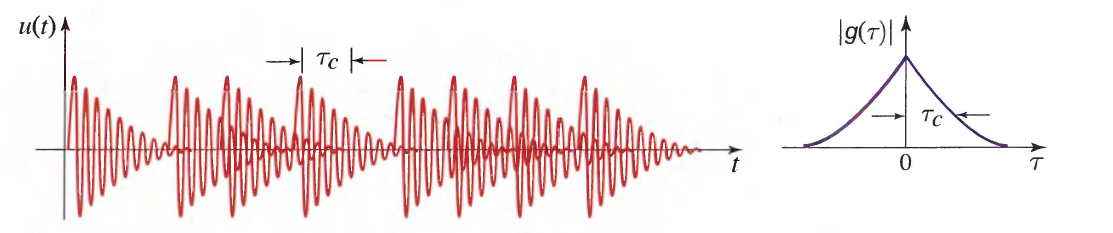
\includegraphics[width=0.9\textwidth]{11_1_6.PNG}
\caption{由在随机时间发射的波包组成的光的相干时间为一个波包的持续时间。}
\label{fig: 11_1_6}
\end{figure}
波包可能是具有指数衰减包络的正弦曲线,譬如,在 $ t = 0 $时刻(给定位置处)发射的波包的复波函数为
\begin{equation}
U_p(t) = 
\begin{cases}
A_p \exp(-\frac{t}{\tau_c}) \exp(j \omega_0 t), & t\geq 0 \\
0, & t < 0 .
\end{cases}
\end{equation}
波包的发射时间是完全随机的,不同次发射的随机、独立的相位包含于$ A_p $中。凭借数学统计学的手段,我们可以通过必要的平均运算来确定整个场的统计性质。譬如我们可以得到整个场的复时间相干度 $ g(\tau) = \exp(- \lvert \tau \rvert / \tau_c) \exp(j \omega_0 \tau) $, $g(\tau)$为一双边指数函数,与之对应的功率频谱密度$ S(\mu) = (\Delta \mu /2 \pi)/ [(\mu - \mu_0)^2 + (\Delta \mu /2)^2] $,轮廓为Lorentzian,其中$ \Delta \mu = 1/ \pi \tau_c $ (见 表 A.2-1 于 Appendix A)。此时,相干时间 $ \tau_c $刚好等于波包的宽度。所以,说这个光在相干时间内是相关的也就是说这个光在单一波包的持续时间内是相关的。\\
\noindent{\crule[ksc]{\textwidth}{0.1cm}}

\bigbreak\begingroup
\color{ksc}
\subsubsection{空间相干性}
\endgroup
\noindent\textcolor{ksc}{\textbf{\textsl{互相干函数}}}\\
函数$ U(r_1,t) $和 $U(r_2,t) $,在一成对位置$ r1 $ 和$ r2 $处的互相关函数,是一个对随机函数$ U(r,t) $的时间和空间涨落的重要描述量。
\begin{equation}
G(r_1, r_2, \tau) = \langle U^\ast (r_1, t) U(r_2, t + \tau) \rangle .
\end{equation}
此以时间延迟$\tau$作为自变量之一的函数称为 \textbf{互相干函数}。其归一化后
\begin{equation}
g(r_1, r_2, \tau) = \frac{G(r_1, r_2, \tau)}{\sqrt{I(r_1) I(r_2)}},
\end{equation} 
称为复相干度。 当两位置重合时有$ r_1 = r_2 = r $,(11.1-21) and (11.1-22)就分别退化为(11.1-4) 和(11.1-7)定义在位置$ r $处的复时间相干函数和复时间相干度。再退化一步,当$ \tau = 0 $时,$ I(r) = G(r, r, 0) $即为位置 $ r $处的光强。
\par 复相干度$ g(r_1, r_2, \tau) $是随机变量 $ U^\ast (r_1, t) $ 与$ U(r_2, t + \tau) $的互相关系数,其绝对值在0到1之间
\begin{equation}
0 \leq \lvert g(r_1, r_2, \tau) \rvert \leq 1 .
\end{equation}
因此$ g(r_1, r_2, \tau) $是$ r_1 $处的涨落,与时间延迟$ \tau $后$ r_2 $处的涨落的相关度的一个测度。
\par 当相量$ U(r_1, t) $与相量 $ U(r_2, t) $是独立涨落的,并且二者的相位都是完全随机的(在0 到 $ 2\pi $内等可能分布),有 $ g(r_1, r_2, \tau) = 0 $,缘于乘积$ U^\ast (r_1, t) U(r_2, t + \tau) $的均值为0。此时,光在两位置处的涨落是不相关的。另一个极限情形是,光在 $ r_1 $和时间延迟$ \tau $后$ r_2 $处的涨落完全相关,此时有 $ g(r_1, r_2, \tau) = 1 $。 注意,$ \lvert g(r_1, r_2, 0) $ 并一定等于1,但根据定义我们可以得到$ g(r, r, 0) = 1 $。
\par $ g(r_1, r_2, \tau) $ 对时间延迟的依赖和位置的依赖描述了光的 时间相干性和空间相干性。图 11.1-7 举例说明了$ g(r_1, r_2, \tau) $对距离$ \lvert r_1 - r_2 \rvert $和时间延迟$ \tau $的依赖性。
\begin{figure}[H]
\centering
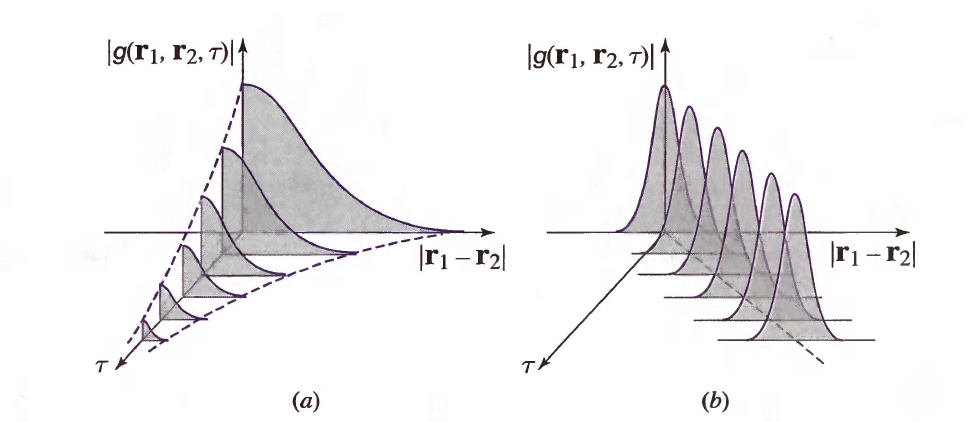
\includegraphics[width=0.9\textwidth]{11_1_7.PNG}
\caption{以距离 $ \lvert r_1 - r_2 \rvert $和时间延迟$ \tau $作为自变量的函数$ g(r_1, r_2, \tau) $ 的两个例子。在 (a) 中,在给定距离 $ \lvert r_1 - r_2 \rvert $时,最大值出现在$ \tau = 0 $处。在(b)中,最大值出现在 $ \lvert r_1 - r_2 \rvert = c \tau $处。}
\label{fig: 11_1_7}
\end{figure}
\par 光的时间涨落和空间涨落是紧密相关的,缘于光是以波的形式传播且复波函数 $ U(r,t) $必须满足波动方程。这就对互相干函数构成了特定约束。为了阐明这一点,考虑一个以速度c,在均匀非色散介质中,沿$ z $ 轴方向传播的随机光平面波。当时间延迟$ \tau = \tau_0 \equiv \lvert z_2 - z_1 \rvert /c $时,点$ r_1 = (0, 0, z_1) $与 点$ r_2 = (0, 0, z_2) $处的涨落是完全相关的,也就是说$ \lvert g(r_1, r_2, \tau_0) \rvert = 1 $。如图 11.1-7(b)所示,以$ \tau $作为自变量之一的函数$ g(r_1, r_2, \tau) $的峰值点出现在 $ \tau = \tau_0 $处。在 Sec. 11.1D中,我们还会再次讨论这个例子。\\
\noindent{\crule[ksc]{\textwidth}{0.2cm}}
\textbf{EXERCISE 11.1-3} \\
\textbf{约束互相干函数的微分方程.}在自由空间中,$ U(r,t) $必须满足波动方程,即 I $ \nabla^2 U - (1/c^2  \partial^2 U / \partial t^2 = 0 $。利用定义(11.1-21)证明互相干函数  $ G(r_1, r_2, \tau) $也满足两个微分方程
\begin{subequations}
\begin{align}
\nabla_1^2 G - \frac{1}{c^2} \frac{\partial^2 G}{\partial \tau^2}  &= 0\\
\nabla_2^2 G - \frac{1}{c^2} \frac{\partial^2 G}{\partial \tau^2 } &= 0,
\end{align}
\end{subequations} 
其中, $ \nabla_1^2 $和$ \nabla_2^2 $分别是对 $ r_1 $ 和 $ r_2 $的 Laplacian算子。\\
\noindent{\crule[ksc]{\textwidth}{0.2cm}}
\bigbreak\noindent\textcolor{ksc}{\textbf{\textsl{互强度}}}\\
我们可以通过考察互相干函数,在固定时间延迟 $ \tau $时,对位置的依赖来评估光的空间相关性。如图 11.1-7(a)中的例子所示,在很多状况下,取固定时间延迟$ \tau = 0 $是最合适的。然而像图 11.1-7(b)中的例子,取$ \tau = 0 $并不总是最合适的。$ \tau = 0 $时,互相干函数
\begin{equation}
G(r_1, r_2, 0) = \langle U_\ast (r_1, t) U(r_2, t) \rangle ,
\end{equation}
称为\textbf{互强度} ,可简单地用$ G(r_1, r_2) $ 表示。互强度的对角值($ r_1 = r_2 = r $时的值) 即为光强) $ I(r) = G(r,r) $。
\par 当研究的光学系统中所遇到的光程差均远小于相干长度$ l_c = c\tau_c $时,我们可认为光是完全时间相干的,故互相干函数是时间的谐波函数
\begin{equation}
G(r_1, r_2, \tau) = G(r_1, r_2) \exp(j\omega_0 \tau),
\end{equation}
其中 $ \nu_0 $ 为中心频率。 此时,我们称该光是\textbf{准单色的},互强度 $ G(r_1, r_2) $也完全描述了空间相干性。
\par 类似地,复相干度在$ \tau = 0 $处的取值$ g(r_1, r_2, 0) $ 可简记为$ g(r_1, r_2) $。因此
\begin{equation}
g(r_1, r_2) = \frac{G(r_1, r_2)}{\sqrt{I(r_1) I(r_2)}}
\end{equation}
即为归一化的互强度。其模$ \lvert g(r_1, r_2) \rvert $的值在0到1之间,可作为时间延迟$ \tau $为0时,空间相干性的一个测度。若复波函数$ U(r, t) $是确定的,对于任意一对位置 $ r_1 $ 和 $ r_2 $ ,均有$ \lvert g(r_1, r_2) = 1\rvert $,即光在各处完全相干。
\bigbreak\noindent\textcolor{ksc}{\textbf{\textsl{相干面积}}}\\
在一给定平面的给定位置$ r_2 $的邻域内,我们用距离$ \lvert r_1 - r_2 \rvert $的函数$ \lvert g(r_1, r_2) \rvert $来描述准单色光的空间相干性。此函数在 $ r_1 = r_2 $时值为1,且随着$ \lvert r_1 - r_2 \rvert $的增大而减小(但并不一定单调)。函数$ \lvert g(r_1, r_2) \rvert $比规定值(譬如,最大值的$ \frac{1}{2} $ 或 $ \frac{1}{e} $)的 $ r_1 $点扫过的面积,称为\textbf{相干面积}。如 图 11.1-8所示,相干面积表示的是,对于一固定点 $ r_2 $, 以$ r_1 $ 为自变量的函数 $ \lvert g(r_1, r_2) \rvert $ 的空间广度。在相干光的理想极限情况下,相干面积为无穷大。
\par 相干面积是描述随机光的一个重要参数,我们必须将其与光学系统的其它相关尺寸放在一起考虑。譬如,若相干面积远大于光阑的大小,则在感兴趣的区域上均有$ \lvert g(r_1, r_2) \rvert \approx 1 $,此时,我们可认为光是相干的,即使光的相干面积有限。类似地,若相干面积比光学系统的分辨率要小得多,则我们可认为相干面积无穷小,即对于实际中任意$ r_1 \neq r_2 $,均有 $ g(r_1, r_2) = 0 $。在这个极限情形下,我们说光是 \textbf{非相干的}。
\par 由扩展热源表面辐射出的光的相干面积与$ \lambda^2 $是一个量级,因此,在大多数实际情况下,可认为这种光是非相干的。所以说,相干和非相干只是代表部分相干的两个极限的理想情况。
 \begin{figure}[H]
\centering
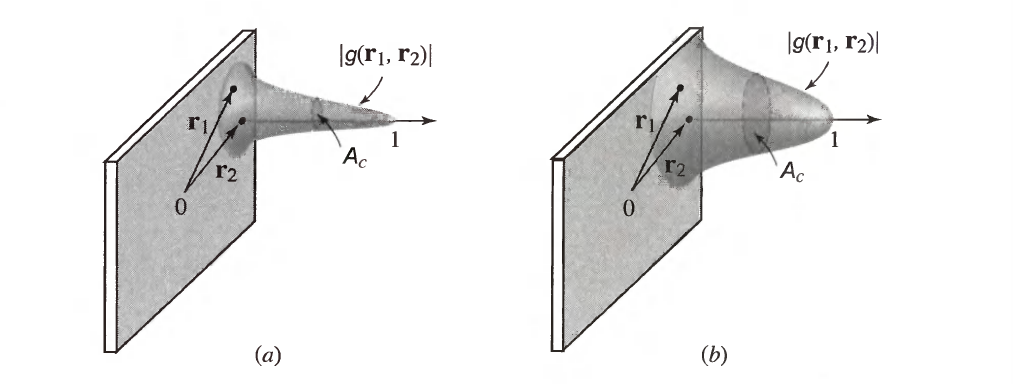
\includegraphics[width=0.9\textwidth]{11_1_8.PNG}
\caption{在固定点 $ r_2 $的邻域内,以$ r_1 $作为自变量的函数——归一化的互强度的模,的两个说明性示例。(a)中的相干面积比(b)中的相干面积要小。}
\label{fig: 11_1_8}
\end{figure}
\bigbreak\noindent\textcolor{ksc}{\textbf{\textsl{互频谱密度}}}\\
互相关函数$ G(r_1, r_2, \tau) $ 描述了任意时间延迟$ \tau $下的空间相关性。我们取$ \tau = 0 $从而定义了互强度$ G(r_1, r_2) = G(r_1, r_2, 0) $,这样定义的互强度适合用来描述准单色光的空间相干性。另一个有效的方法是,通过考察某一固定频率处的空间相关性,而在频域中描述相干性。我们定义\textbf{互频谱密度}(或者称互功率频谱密度)为$ G(r_1, r_2, \tau) $以$ \tau $作积分变量的傅里叶变换:
\begin{equation}
S(r_1, r_2, \nu) = \int_{-\infty}^{+\infty}G(r_1, r_2, \tau) \exp(-j2\pi \nu \tau) \dif \tau .
\end{equation}
当$ r_1 = r_2 = r $时,互频谱密度退化为(11.1-17)中定义的在位置 $ r $处的频谱密度。
\par 归一化的互频谱密度定义为
\begin{equation}
s(r_1, r_2, \nu) = \frac{S(r_1, r_2, \nu)}{\sqrt{S(r_1, r_1, \nu)S(r_2, r_2, \nu)}} ,
\end{equation}
其模可被证明在0到1之间,故归一化的互频谱密度可作为频率 $ \nu $处的空间相干度的测度。互频谱密度代表了频率为 $ \nu $的成分,在位置$ r_1 $ 、$ r_2 $处的涨落的相关度。
\par 在特定情况下,光的互频谱密度可因式分解成一位置的函数与另一频率的函数的乘积,即$ S(r_1, r_2, \nu) = G(r_1, r_2) s(\nu) $,故其空间性质与频谱性质是可分离的,此时我们称光是\textbf{互谱纯的}。与此同时,其对应的互相干函数也一定能因式分解成一位置的函数与另一时间的函数的乘积,即 $ G(r_1, r_2, \tau) = G(r_1, r_2) g(\tau) $,其中,$ g(\tau) $为 $ s(\nu) $的逆傅里叶变换。若合适地选取分解得到的因式前的系数,使得 $ \int s(\nu) \dif \nu = 1 $,便可知 $ G(r_1, r_2) = G(r_1, r_2, 0) $,显然这里的 $G(r_1, r_2) $不是别的正是互强度。互谱纯的光有两个重要的性质:
\par 1. 在单一位置 $ r $处, $ S(r, r, \nu) = G(r, r) s(\nu) = I(r) s(\nu) $。频谱在任意位置处的轮廓均相同。若这个光代表一个可见图像,则这个图像各处颜色相同,亮度可能不同。
\par 2. 归一化的互频谱密度
\begin{equation}
s(r_1, r_2, \nu) = G(r_1, r_2) / \sqrt{G(r_1, r_1) G(r_2, r_2)} = g(r_1, r_2)
\end{equation}
与频率无关,此时,归一化的互强度 $ g(r_1, r_2) $描述了所有频率处的空间相干性。

\bigbreak\begingroup
\color{ksc}
\subsubsection{纵向相干性}
\endgroup
在这一节中,我们通过介绍具有固定波前的随机波(譬如平面波和球面波)的例子,来介绍轴向相干性的概念。
\bigbreak\noindent\textcolor{ksc}{\textbf{\textsl{部分相干平面波}}}\\
考虑一以速度c,在均匀介质中,沿$z$轴方向传播的平面波
\begin{equation}
U(r, t) = a (t - \frac{z}{c}) \exp[j\omega_0 ((t - \frac{z}{c})]
\end{equation}
如 Sec. 2.6A中所示, $ a(t) $可取任意函数,$ U(r,t) $ 均满足波动方程。若$ a(t) $ 是随机函数,则$ U(r,t) $代表部分相干光。(11.1-21)定义的互相干函数此时可化为
\begin{equation}
G(r_1, r_2, \tau) = G_a (\tau - \frac{z_2 - z_1}{c}) \exp [j\omega_0 (\tau - \frac{z_2 - z_1}{c})] ,
\end{equation}
其中,$ z_1 $ 、$ z_2 $分别表示$ r_1 $ 、$ r_2 $在$z$方向的分量,$G_a (\tau) = \langle a^\ast (t) a(t + \tau) \rangle $为时间t无关的$ a(t) $的自相关函数。
\par 光强$ I(r) = G(r, r, 0) = G_a (0) $是常数。时间相干函数$ G(r, r, \tau) = G_a (\tau) \exp (j\omega_0 \tau) $只是时间的函数而与位置无关。复时间相干度$ g(r, r, \tau) = g_a (\tau) \exp(j\omega_0 \tau) $ ,其中$ g_a (\tau) = G_a (\tau) / G_a (0) $。$ \lvert g_a (\tau) \rvert = \lvert g(r, r, \tau) \rvert $的宽度也就等于 (11.1-10)中定义的$\lvert g(r) \rvert$的宽度,即为相干时间$ \tau_c $。显然其相干时间在各个位置均相等。
\par 功率频谱密度$ S(\nu) $是时间相干函数 $ G(r, r, \tau) $的傅里叶变换,故由$ G(r, r, \tau) = G_a (\tau) \exp (j\omega_0 \tau) $可以看出,$ S(\nu) $等于$ G_a (\tau) $的傅里叶变换平移 $ \nu_0 $ 后的结果(见傅里叶变换的频移性质于 Appendix A, Sec. A.1.) 因此,该波在空间的各个位置都有相同的功率频谱密度。
\par 该波用来描述空间相干性的互强度可化为
\begin{equation}
G(r_1, r_2, 0) = G_a (\frac{z_1 - z_2}{c}) \exp[j\omega_0 \frac{z_1 - z_2}{c}]
\end{equation}
归一化后可得
\begin{equation}
g(r_1, r_2, 0) = g_a (\frac{z_1 - z_2}{c}) \exp[j\omega_0 \frac{z_1 - z_2}{c}]
\end{equation}
若两点 $ r_1 $、$ r_2 $位于同一横截面上,也即 $ z_1 = z_2 $,则可得到$ \lvert g(r_1, r_2, 0) \rvert = \lvert g_a (0) = 1 $。这就是说,在同一波前(垂直于z轴的平面)上的任意两点都是完全相关的,任意横截面上的相干面积都是无穷大(图 11.1-9)。另一方面,若两点的轴向距离 $ z_2 - z_1 $  满足$ \lvert z_2 - z_1 \rvert / c > \tau_c $或 $ \lvert z_2 - z_1 \rvert > l_c $,其中,$ l_c = c\tau_c $为相干长度,则两点几乎是不相干的。
 \begin{figure}[H]
\centering
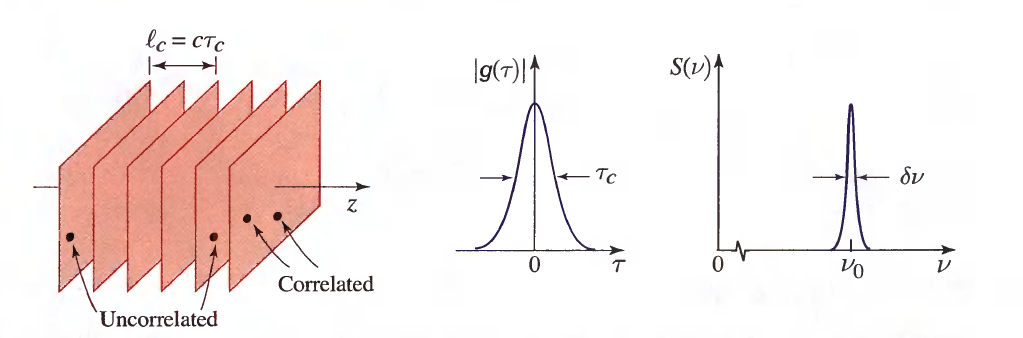
\includegraphics[width=0.9\textwidth]{11_1_9.PNG}
\caption{部分相干平面波在任意波前(横截面)上的两点的涨落,均完全相关。而在轴向距离大于相干长度 $ l_c = c \tau_c $的两波前上的两点,涨落几乎是不相关的。}
\label{fig: 11_1_9}
\end{figure}
\par 总而言之:部分相干平面波在任意横截面上是空间相干的,在轴向方向上是空间部分相干的,其轴向(纵向)空间相干性与时间相干性存在一对一的关系。对于部分相干平面波而言,相干长度$ l_c = c\tau_c $与系统中遇到的最大光程差$ l_{max} $的比值,决定了对其相干性的判断。若 $ l_c \gg l_{max} $,则我们认为其是完全相干的。表 11.1-2列出了一些光源的相干长度。
\bigbreak\noindent\textcolor{ksc}{\textbf{\textsl{部分相干球面波}}}\\
我们用下面的复波函数来表示部分相干球面波 (见 Sec. 2.2B 和 Sec. 2.6A)
\begin{equation}
U(r, t) = \frac{1}{r} a(t - \frac{r}{c}) \exp[j\omega_0 (t - \frac{r}{c})],
\end{equation}
其中,$ a(t) $ 为一随机函数。部分相干球面波对应的互相干函数为
\begin{equation}
G(r_1, r_2, \tau) = \frac{1}{r_1 r_2} G_a (\tau - \frac{r_2 - r_1}{c}) \exp [j\omega_0 (\tau - \frac{r_2 - r_1}{c})],
\end{equation}
其中, $ G_a (\tau) = \langle a^\ast (t) a(t+ \tau) \rangle $。
\par 部分相干球面波的光强$ I(r) = G_a (0) / r^2 $以平方反比定律变化。相干时间$ \tau_c $,即函数$ \lvert g_a (\tau) \rvert = \lvert G_a (\tau) / G_a (0) \rvert $的宽度,在空间各点处均相等。功率频谱密度$S(\nu, \tau) = S_a (\nu - \nu_0) / r^2$在任意波前上的相等,其中,$S_a(\nu)$为$G_a (\tau)$的傅里叶变换。归一化后的互强度$g(r_1, r_2) = g_a (\frac{r_1 - r_2}{c})\exp [j\omega_0 \frac{r_1 - r_2}{c}]$,故同一波前(球面)上任意两点的涨落是完全空间相关的,径向距离为$ \lvert r_2 -r_1 \rvert \gg l_c = c\tau_c $的两波前上的点的涨落,几乎是不相关的(见 图 11.1-10)。
\par 任意一个通过小孔的部分相干波都会变成部分相干球面波,因此这个过程赋予了产生的波空间相干性(以小孔为球心的任意球面上的两点是完全空间相关的),其径向空间相干性与时间相干性也存在一对一的关系。然而,产生的球面波,与未通过小孔前的波一样,仍然是时间部分相干的。故小孔只赋予了波空间相干性,而没有赋予其时间相干性。
\par 假设我们在小孔上放一窄带宽的光滤波片,则通过小孔的光便几乎是单色的。此时波不但获得了空间相干性,也获得了完全时间相干性。窄带滤波片(作为频域滤波器)引入了时间相干性,小孔(作为空域滤波器)引入了空间相干性。当然,获得这种理想的波是以时域和空域滤波带来的光能损失为代价的。
 \begin{figure}[H]
\centering
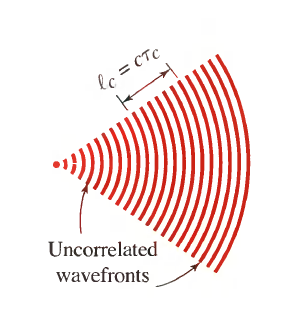
\includegraphics[width=0.3\textwidth]{11_1_10.PNG}
\caption{部分相干球面波在同一波面上的两点是完全空间相干的,而在径向距离远大于相干长度的两波面上的点是几乎空间不相干的。}
\label{fig: 11_1_10}
\end{figure}

\bigbreak\begingroup
\color{ksc}
\subsection{部分相干光的干涉}
\endgroup
我们已经在 Sec. 2.5讨论了相干光的干涉,本节致力于讨论部分\textsl{相干}光的干涉。
\bigbreak\begingroup
\color{ksc}
\subsubsection{两个部分相干波的干涉}
\endgroup
两个部分相干波$ U_1 $、$ U_2 $的统计特性,不仅包括各自的互相干函数,也包括两波涨落之间的相关度的测度。在给定位置$ r $和给定时间$ t $时,两波的光强分别为$ I_1 = \langle \lvert U_1 \rvert ^2 \rangle $和$ I_2 = \langle \lvert U_2 \rvert ^2 \rangle $,我们用统计平均值$ G_{12} = \langle U_1^\ast U_2 \rangle $来描述两波的互相关性,其归一化后的形式为
\begin{equation}
g_{12} = \frac{\langle U_1^\ast U_2 \rangle}{\sqrt{I_1 I_2}} .
\end{equation}
\par 当两波发生叠加,叠加后的平均强度为
\begin{align}
I = & \langle \lvert U_1 + U_2 \rvert ^2 \rangle = \langle \lvert U_1 \rvert ^2 \rangle + \langle \lvert U_2 \rvert ^2 \rangle + \langle U_1^\ast U_2 \rangle + \langle U_1 U_2^\ast \rangle \notag \\
={} & I_1 + I_2 + G_{12} + G_{12}^\ast = I1 + I2 + 2 Re\{ G_{12} \} \notag \\
={} & I_1 + I_2 + 2\sqrt{I_1 I_2}Re\{ g_{12} \},
\end{align}
可知
\begin{equation}
I = I_1 + I_2 + 2\sqrt{I_1 I_2} \lvert g_{12} \rvert \cos \varphi ,
\end{equation}
其中,$ \varphi = arg\{ g_{12} \} $ 是 $ g_{12} $的相位。(11.2-3)中等式右边的第三项代表光干涉。 
\par 考虑一下两个重要的极限情况
\bigbreak\par 1. 若两波是完全相关的,则有 $ g_{12} = \exp (j\varphi) $,$ \lvert g_{12} \rvert = 1 $,(11.2-3)退化为两个相位差为 $ \varphi $的相干波的干涉公式(2.5-4)。
\bigbreak\par 2. 若两波是不相关的,则 $ g_{12} = 0 $,(11.2-3)简化为 $ I = I_1 + I_2 $,也就没有发生干涉。
\bigbreak\par 一般情况下,如图 11.2-1所示,归一化(均值为1)的光强 $ I $与相位$ \varphi $的关系具有正弦曲线的形式。干涉的强度可以用\textbf{可见度} $ \mathcal{V} $(也称为调制深度或干涉条纹的对比度)来衡量
\begin{equation}
\mathcal{V} = \frac{I_{max} - I_{min}}{I_{max} + I_{min}},
\end{equation}
其中,$ I_{max} $和$ I_{min} $分别为 $ I $随$ \varphi $变化时取到的最大值和最小值。$ \cos \varphi $的取值为1到-1,将 (11.2-3)代入(11.2-4)可得
\begin{equation}
\mathcal{V} = \frac{2\sqrt{I_1 I_2}}{I_1 + I_2} \lvert g_{12} \rvert .
\end{equation}
不难看出,可见度正比于归一化的互相关 $ \lvert g_{12} \rvert $。特别地,当 $ I_1 = I_2 $时,有
\begin{equation}
\mathcal{V} = \lvert g_{12} \rvert .
\end{equation}
 \begin{figure}[H]
\centering
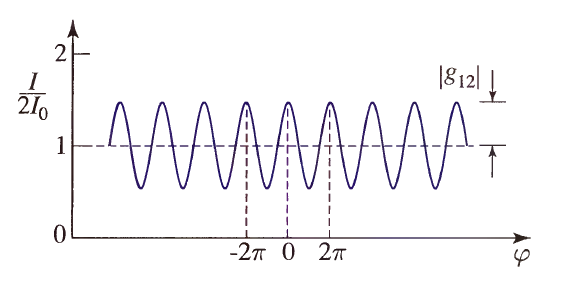
\includegraphics[width=0.3\textwidth]{11_2_1.PNG}
\caption{由两个等光强($ I_1 = I_2 = I_0 $)的部分相干光叠加,得到的光的归一化后的光强,其为归一化后的互相关$ g_{12} $的相位$ \varphi $的函数。这个正弦条纹的可见度$ \mathcal{V} = \lvert g_{12} \rvert $.}
\label{fig: 11_2_1}
\end{figure}
\par 我们会在大量特定的场景下,利用相干公式(11.2-3),讨论时间相干性和空间相干性对部分相干光干涉的影响。
 
\bigbreak\begingroup
\color{ksc}
\subsubsection{干涉与时间相干性}
\endgroup
考虑一部分相干波$ U(t) $,其强度为$ I_0 $,复时间相干度为 $ g(\tau) = \langle U^\ast (t) U(t + \tau) \rangle / I_0 $。若$ U(t) $与其自身在延迟时间 $ \tau $后的拷贝$ U(t + \tau) $发生叠加,则叠加后的波的强度$ I $为多少?
\par 利用干涉公式(11.2-2),并将$ U_1 = U(t) $, $ U_2 = U(t + \tau) $, $ I_1 = I_2 = I_0 $以及$ g_{12} = \langle U_1^\ast U_2 \rangle / I_0 = \langle U^\ast U(t + \tau) \rangle / I_0 = g(\tau) $代入,可得
\begin{equation}
I = 2 I_0 [1 + Re\{g(\tau)\}] = 2 I_0 [1 + \lvert g(\tau) \rvert \cos \varphi (\tau)],
\end{equation}
其中, $ \varphi (\tau) = arg\{g(\tau)\}$。显然,波$ U(t) $的复时间相干度在时刻$\tau$的值,决定了该波与其自身在延迟时间 $ \tau $后的拷贝$ U(t + \tau) $发生干涉的能力。
\par 我们可以使用如下手段,来实现波与其自身时间延迟后的拷贝进行叠加:使用一分束器将波分为相同的两束,其中一束光比另一束光经过的光程要长,再在另一个(或同一个)分束器上重新合到一起。譬如,我们使用一个Mach-Zehnder或Michelson干涉仪(见 图 2.5-3)就可以完成上述操作。
\par 考虑一个Sec. 11.1D [见 (11.1-31)]介绍的部分相干平面波的例子,其复时间相干度为$ g(\tau) = g_a (\tau) \exp(j\omega_0 \tau) $,频谱宽度为$ \Delta \nu_c = 1 / \tau_c $,其中,$ \tau_c $($ \lvert g_a (\tau) \rvert $的宽度)为相干时间。代入(11.2-7),可得
\begin{equation}
I = 2 I_0 \{1 + \lvert g_a (\tau) \rvert \cos [\omega_0 \tau + \varphi_a (\tau)]\} ,
\end{equation}
其中,$ \varphi_a (\tau) = arg \{g_a (\tau)\} $。
\par 图 11.2-2 给出了 $ I $ 与 $ \tau $之间的关系,即\textbf{干涉图}。 干涉图在某一特定时间延迟$ \tau $的邻域内的可见度为$ \mathcal{V} = \lvert g(\tau) \rvert = \lvert g_a (\tau) \rvert $。可见度在$ \mathcal{V}$在$ \tau = 0 $ 时取得峰值1,且在$ \tau \gg \tau_c $ 时(即光程差远大于相干长度$ l_c = c\tau_c $),几乎为0。对于图 11.2-2 所示的Michelson干涉仪而言,$\tau = 2(d_2 - d_1) / c $,仅当光程差小于相干长度时干涉才会发生。
 \begin{figure}[H]
\centering
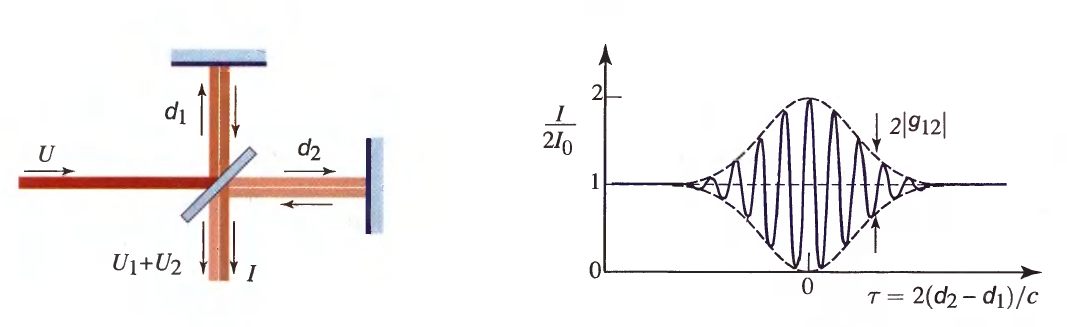
\includegraphics[width=0.9\textwidth]{11_2_2.PNG}
\caption{在Michelson干涉仪中,以部分相干平面波作为入射光时,得到的以时间延迟$ \tau $作为自变量的归一化后的强度$ I / 2I_0 $。可由干涉图的可见性来确定光的复时间相干度的模。}
\label{fig: 11_2_2}
\end{figure}
\par 因此,我们可以通过检测干涉图案的可见性(作为一时间延迟的函数),来测量一个波的复时间相干度的模$\lvert g(\tau) \rvert $。 $ g(\tau) $的相位可以通过观察干涉图峰值点的位置得到。
\bigbreak\noindent\textcolor{ksc}{\textbf{\textsl{傅里叶变换光谱学}}}\\
将 (11.2-7)写成用波的功率频谱密度$ S(\nu) $表示的形式可以令人发省。利用$ G(\tau) $ 与 $ S(\nu) $之间的傅里叶变换关系,我们有
\begin{equation}
G(\tau) = I_0 g(\tau) = \int_0^\infty S(\nu) \exp(j2\pi\nu\tau) \dif \nu ,
\end{equation}
代入(11.2-7), 并注意到 $ S(\nu) $是实函数且$ \int_0^\infty S(\nu) \dif \nu = I_0 $, 我们有
\begin{equation}
I = 2\int_0^\infty S(\nu) [1 + \cos(2\pi\nu\tau)] \dif \nu .
\end{equation}
此等式的右边,可看成是波的每个单色成分产生的干涉图的加权叠加。每个频率为$ \nu $的成分产生一个周期为 $ 1 / \nu $、可见度为1的干涉图,复合的干涉图由于不同周期的干涉图发生叠加,而呈现出更差的可见度。
\par 等式(11.2-10) 表明,我们可以通过测量得到干涉图$ I $与 $ \tau $的关系,然后利用傅里叶变换的方法转化结果得到频谱密度 $ S(\nu) $ 。这个技术称为\textbf{傅里叶变换光谱学}。
\bigbreak\noindent\textcolor{ksc}{\textbf{\textsl{光学相干断层扫描}}}\\
\textbf{光学相干断层扫描} (optical coherence tomography,OCT) 是一种用于分析多层介质的干涉技术,即测量多层介质的每个边界的反射率和深度。光学相干断层扫描需要一个具有短相干长度的部分相干光源,和一个Michelson干涉仪。如图 11.2-3 所示,一个被可移动的镜子延时后的原始波的一份拷贝,与一系列从样本的多个边界反射回来的波进行叠加。随着可移动的镜子发生平移,探测器测量到的光强,即干涉图,携带了物体的轮廓信息。由于光源的相干长度较短,故干涉图是由一系列中心在$\tau_i$处的条纹组成的,其中,条纹中心$\tau_i$分别对应于可移动镜子的光程延迟与各反射边界的光程延迟相等的时刻。
 \begin{figure}[H]
\centering
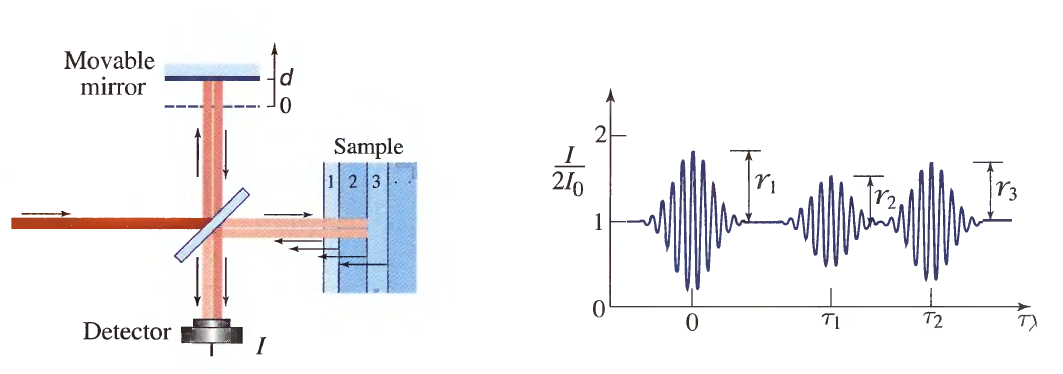
\includegraphics[width=0.9\textwidth]{11_2_3.PNG}
\caption{光学相干断层扫描}
\label{fig: 11_2_3}
\end{figure}
\par 我们记从可移动镜子表面反射回的波为$U(t - \tau) $,记从样本的第 $i$个边界反射回的波为$ r_i U(t - \tau_i), i = 1, 2, ..., $,其中$ r_i $表示第 $i$个边界的振幅反射率,$\tau_i $为第$i$个边界对应的时间延迟。若分束器是对称的,则平均光强为$ I(\tau) = \langle \lvert U(t - \tau) + \sum_i r_i U(t - \tau_i) \rvert ^2 \rangle $,归一化后可得
\begin{equation}
I / 2I_0 = 1 + \sum_i r_i Re\{g(\tau - \tau_i)\} + \sum_{ij} r_i r_j^\ast Re\{g(\tau_j - \tau_i)\} ,
\end{equation}
其中,$ g(\tau) = \langle U^\ast (t) U(t + \tau)\rangle / \langle U^\ast (t) U(t) \rangle $为光源的复时间相干度。
\par (11.2-11)右边的第二项至关重要,因为其代表了从可移动镜子表面反射回的参考光。与从样本的各个边界反射回的光的干涉。(11.2-11)右边的第三项代表的是从样本的各个边界反射回的光之间的干涉,由于这一项与可移动镜子带来的时间延迟 $ \tau = d / c $无关,故可将其当作背景光的一部分并忽略。
\par 对于一个中心频率为 $ \nu_0 $的光源,可知$ g(\tau) = g_a (\tau) \exp(j\omega_0 \tau) $,其中$ g_a (\tau) $ 的宽度即为相干时间$ \tau_c $。此时等式(11.2-11)可化为
\begin{equation}
I / 2I_0 \approx 1 + \sum_i r_i \lvert g_a (\tau - \tau_i) \rvert \cos [\omega_0 (\tau - \tau_i) + \varphi_a (\tau - \tau_i)] ,
\end{equation}
其中, $ \varphi_a (r) = arg\{g_a ( \tau )\} $.。由于光源的相干时间较短,故函数$ g_a (\tau) $较窄。如图 11.2-3所示,从样本的每个边界反射回的光,分别与参考光形成了一个个分开的、持续时间$ \tau_c $较短的、中心为相应时间延迟的干涉条纹。因此,我们可以通过测量OCT干涉图来确定样品每个边界的反射率和每一层的厚度。
\par 光学相干断层扫描已在临床医学和工程学中被证明是一项有效的成像技术。
\bigbreak\begingroup
\color{ksc}
\subsubsection{干涉与空间相干性}
\endgroup
空间相干性对干涉的影响可以用杨氏双孔干涉实验(Exercise 2.5-2中讨论了相干光的情况)来说明。考虑一部分相干光$ U(r,t) $,照在一带有两个分别位于 $ r_1 $ 和 $ r_2 $处的小孔的不透明屏幕上,光的互相干函数为 $ G(r_1, r_2, \tau) = \langle U^\ast(r_1, t) U(r_2, t+\tau) \rangle $ ,复相干函数为 $ g(r_1, r_2, \tau) $。将光强看成是$x$的函数,两个小孔所张的角度$ \theta \approx 2a / d $是一重要的几何参数。
 \begin{figure}[H]
\centering
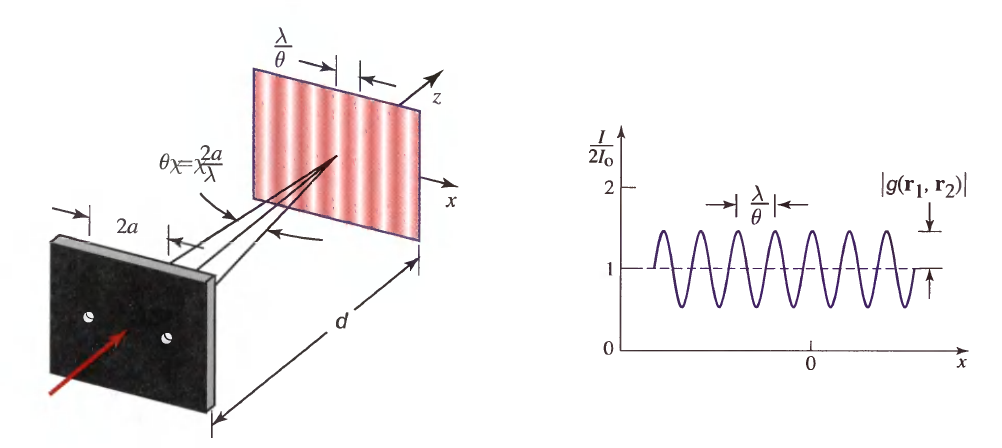
\includegraphics[width=0.9\textwidth]{11_2_4.PNG}
\caption{杨氏双孔干涉仪。入射光是准单色的且在两小孔处归一化的互强度为 $ g(r_1, r_2) $。在远距离的观察平面上,归一化的光强$ I / 2 I_0 $是一周期为$\lambda / \theta $,可见度为$ \mathcal{V} = \lvert g(r_1, r_2) \rvert $,以$x$作为自变量的正弦函数。}
\label{fig: 11_2_4}
\end{figure}
\par 在抛物线(Fresnel)近似的条件下[见 (2.2-17)],两衍射的球面波与$ U(r, t) $的关系可近似为
\begin{subequations}
\begin{align}
U_1 (r, t) \propto U(r_1, t - \frac{\lvert r- r_1 \rvert}{c})  &\approx U(r_1, t - \frac{d + (x+a)^2 / 2d}{c})\\
U_2 (r, t) \propto U(r_2, t - \frac{\lvert r- r_2 \rvert}{c})  &\approx U(r_2, t - \frac{d + (x-a)^2 / 2d}{c}),
\end{align}
\end{subequations} 
二者光强几乎相等,即$ I_1 = I_2 = I_0 $。两波在位置$r$处归一化的互相关为
\begin{equation}
g_{12} = \frac{\langle U_1^\ast (r, t) U_2 (r, t) \rangle}{I_0} = g(r_1, r_2, \tau_x),
\end{equation}
其中,
\begin{equation}
\tau_x = \frac{\lvert r - r_1 \rvert - \lvert r - r_2 \rvert}{c} = \frac{(x + a)^2 - (x - a)^2}{2dc} = \frac{2ax}{dc} = \frac{\theta}{c}x
\end{equation}
为两波相遇时的时间延迟差。
\par 将(11.2-14)代入干涉公式(11.2-3),便可得到观察到的光强 $ I \equiv I(x) $:
\begin{equation}
I(x) = 2 I_0 [1 + \lvert g(r_1, r_2, \tau_x) \rvert \cos \varphi_x] ,
\end{equation}
其中 $ \varphi_x = arg\{g(r_1, r_2, \tau_x)\}$。此等式用波在两小孔处、时间延迟 $ \tau_x = \theta_x / c$时的复相干度的模和相位,描述了观察面上以位置$x$作为自变量的光强图案。
\bigbreak\noindent\textcolor{ksc}{\textbf{\textsl{准单色光}}}\\
若光是中心频率为$ \nu_0 = \omega_0 / 2\pi$的准单色光,即有$ g(r_1, r_2, \tau_x) \approx g(r_1, r_2) \exp (j\omega_0 \tau_x) $,则(11.2-16)可化为
\begin{equation}
I(x) = 2 I_0 [1 + \mathcal{V} \cos (\frac{2\pi \theta}{\lambda}x + \varphi)] ,
\end{equation}
其中 $ \lambda = c / \nu_0, \mathcal{V} = \lvert g(r_1, r_2) \rvert, \tau_x = \theta x / c $, and $ \varphi = arg\{g(r_1, r_2)\}$。此时,干涉条纹是空间周期为 $ \lambda / \theta $ ,可见度为$ \mathcal{V} $的正弦函数。类似于波与自身延时后的拷贝干涉的情形,此干涉图案的可见度 ,等于波在两小孔处归一化的互强度的模(图 11.2-4)。干涉条纹的峰值位置取决于相位$\varphi$。
\bigbreak\noindent\textcolor{ksc}{\textbf{\textsl{扩展光源发出的光的干涉}}}\\
若杨氏干涉仪中的入射波为沿$z$轴传播的相干平面波$ U(r,t) = \exp(-jkz) \exp(j\omega_0 t) $,则有 $ g(r_1, r_2) = 1 $,即 $ \lvert g(r_1, r_2) \rvert = 1 $且$ arg\{g(r_1, r_2) = 0\} $。故此时相干图案的可见度为1,有一峰值在$ x = 0 $处。但若照明光是,沿一在$x-z$平面与z轴夹一小角度 $\theta_x$方向,传播的倾斜平面波,即 $ U(r,t) \approx \exp[-j(kz + k\theta_x x)] \exp (j\omega_0 t) $,则可得到$ g(r_1, r_2) = \exp(-jk\theta_x 2a) $。干涉图案的可见性仍然是1,但倾斜产生了一个相位平移$ \varphi = -k\theta_x 2a = -2\pi \theta_x 2a / \lambda $,故干涉图案横向移动了一个周期的$ 2a \theta_x / \lambda $。当 $ \varphi = 2\pi $时,干涉图案横向移动了一个周期。
\par 现在,假设入射光是,与小孔所在平面张角为 $ \theta_s $的光源,发出的一系列独立平面波(图 11.2-5),则相位平移$ \varphi $便落在范围$ \pm 2\pi (\theta_s / 2) 2a \lambda = \pm 2\pi \theta_s a / \lambda $内,干涉条纹是多个移位后的正弦曲线的叠加。若$ \theta_s = \lambda / 2a $,则$\varphi$的变化范围为$ \pm \pi $,这足够“冲洗掉”干涉图案,使其可见度降至0。
\begin{figure}[H]
\centering
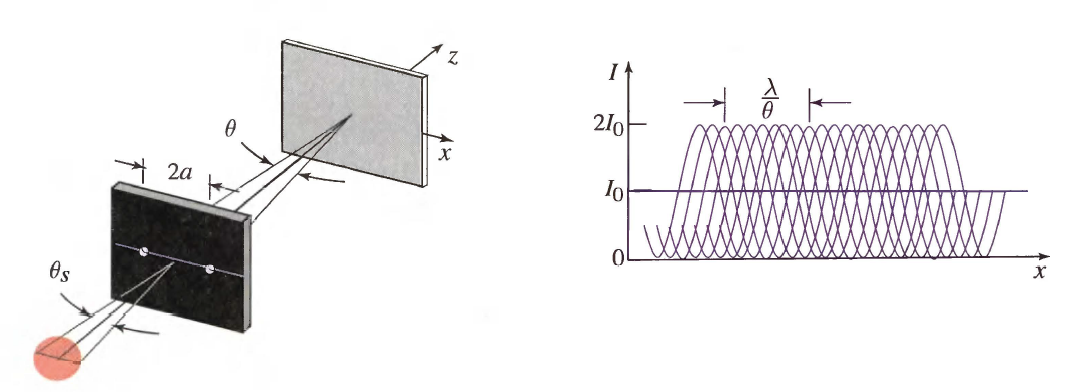
\includegraphics[width=0.9\textwidth]{11_2_5.PNG}
\caption{当使用角直径 $ \theta_s > \lambda / 2a $的光源作为照明光源时,杨氏干涉图案被“冲洗掉”了。当距离$2a$小于$ \lambda / \theta_s $时,条纹变得可见。}
\label{fig: 11_2_5}
\end{figure}
\par 我们认为,当光源的张角$ \theta_s = \lambda / 2a $(或者更大),光在两小孔处空间相干度非常小。因此,距离
\begin{equation}
\rho_c \approx \frac{\lambda}{\theta_s}
\end{equation}
是小孔平面上相干距离的一个测度,
\begin{equation}
A_c \approx (\frac{\lambda}{\theta_s})^2
\end{equation}
为从张角为$\theta_s$的光源发出的光的相干面积的一个测度。譬如,太阳的张角为 $0.5 \degree$,故滤波后波长为$\lambda$的太阳光的相干距离为$\rho_c \approx \lambda / \theta_s \approx 115\lambda$。当 $\lambda = 0.5 \mu m$时,$, \rho_c \approx 57.5 \mu m$。更加严格的分析 (见 Sec. 11.3C)表明,具有均匀光强的、圆形非相干光源的相干距离为
\begin{equation}
\rho_c = 1.22 \frac{\lambda}{\theta_s} .
\end{equation}
\bigbreak\noindent\textcolor{ksc}{\textbf{\textsl{频谱宽度对干涉的影响}}}\\
最后,我们考察在杨氏双孔干涉仪中,频谱宽度对干涉的影响。我们认为,入射波的功率频谱密度是中心在$\nu_0$,宽度为$\Delta \nu_c$的窄宽函数,其中$\Delta \nu_c \ll \nu_0$。此时,复相干度具有下面的形式
\begin{equation}
g(r_1, r_2, \tau) = g_a (r_1, r_2, \tau) \exp (j\omega_0 \tau),
\end{equation}
其中,$g_a (r_1, r_2, \tau)$为一随$\tau$变化而缓慢变化的函数(相比于周期$1 / \nu_0$而言)。将(11.2-21)代入(11.2-16),可得
\begin{equation}
I(x) = 2I_0 [1 + \mathcal{V}_x \cos(\frac{2\pi \theta}{\overline{\lambda}} + \varphi_x)] ,
\end{equation}
其中, $\mathcal{V}_x = \lvert g_a (r_1, r_2, \tau_x) \rvert , \varphi_x = arg\{g_a (r_1, r_2, \tau_x)\} , \tau_x = \theta x / c$, $\overline{\lambda} = c / \nu_0$。
\par 因此,干涉图案是一周期为 $\overline{\lambda} / \theta$的正弦波,其可见度$\mathcal{V}_x$和相位$\varphi_x$分别等于两小孔处,时间延迟为 $\tau_x = \theta x / c$时,复相干度的模和相位。 若 $\lvert g_a(r_1, r_2, \tau) \rvert$在$\tau = 0$时等于1,随$\tau$的增大而减小且当 $\tau \gg \tau_c$时趋于0,则可见度 $\mathcal{V}_x $ 在 $x =0$时等于1,随$x$的增大而减小,当$x \gg x_c = c\tau_c / \theta$时趋于0。故干涉图案在距离 
\begin{equation}
x_c = \frac{l_c}{\theta} , 
\end{equation}
内可见,其中, $l_c = c\tau_c$ 为相干长度,$\theta$为两小孔的张角(图 11.2-6)。
\begin{figure}[H]
\centering
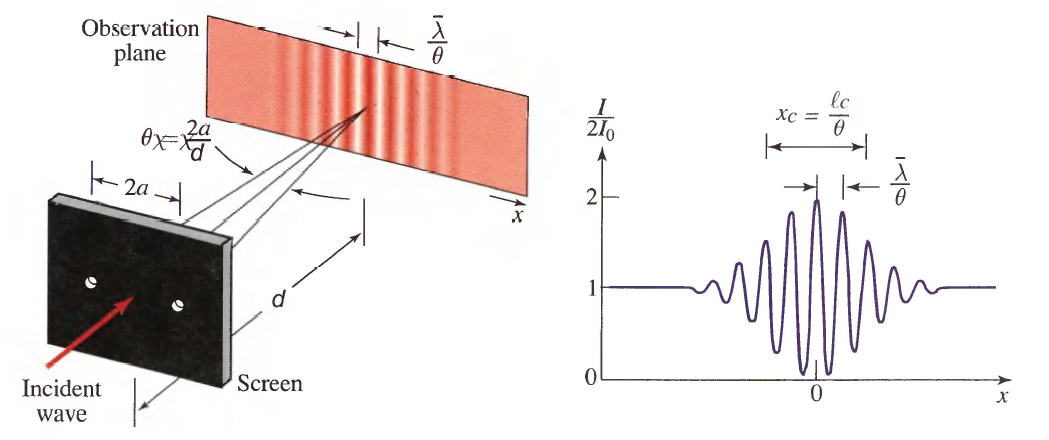
\includegraphics[width=0.9\textwidth]{11_2_6.PNG}
\caption{杨氏干涉条纹的可见度 $\mathcal{V}_x $等于两小孔处,时间延迟为 $\tau_x = \theta x / c$时,复相干度的模。对于空间部分相干光而言,可观察到的条纹数等于相干长度与中心波长的比值,或者等于中心频率与频谱宽度的比值。}
\label{fig: 11_2_6}
\end{figure}
\par 因此,可观察到的条纹数为$x_c / (\overline{\lambda} / \theta) = l_c / \overline{\lambda} = c\tau_c / \overline{\lambda} = \nu_0 / \Delta \nu_c$。其等于相干长度与中心波长的比值$l_c / \overline{\lambda}$,或者中心频率与频谱宽度的比值 $\nu_0 / \Delta \nu_c$。显然,若$\lvert g(r_1, r_2, 0) \rvert < 1$,即光源不是空间相干的,则可见性会进一步下降,能观察到的条纹会更少。

\bigbreak\begingroup
\color{ksc}
\subsection{部分相干光在光学系统中的传播}
\endgroup
我们已经在第二章和第四章讨论了相干光通过薄光学元件、光阑、自由空间时的传播,本节,我们仍然研究这些情形下光的传播,不过将主体换为准单色部分相干光。我们认为,频谱宽度足够小以致相干长度 $l_c = c\tau_c = c / \Delta \nu_c$比系统中的所有光程差都大得多。此时,互相干函数可近似为 $G(r_1, r_2, \tau) \approx G(r_1, r_2) \exp(j\omega_0 \tau)$,其中,$G(r_1, r_2)$为互强度,$\nu_0$为中心频率。
\par 在一开始我们需要指出:适用于确定函数 $U(r)$(代表相干光)的传播规律同样也适用于随机函数$U(r)$(代表部分相干光)。然而,对于部分相干光而言,我们感兴趣的是那些约束统计平均值(光强$I(r)$和互强度$G(r_1, r_2)$)的定律。

\bigbreak\begingroup
\color{ksc}
\subsubsection{部分相干光的传播}
\endgroup
\bigbreak\noindent\textcolor{ksc}{\textbf{\textsl{通过薄光学元件的传播}}}\\
当一个部分相干波通过一复振幅透过率为$t(x,y)$的薄光学元件时,入射波和透射波满足 $U_2 (t) = t(r) U_1 (r)$的关系,其中, $r = (x,y)$代表元件平面的位置(见图 11.3-1)。利用互强度的定义 $G(r_1, r_2) = \langle U^\ast (r_1) U(r_2) \rangle$,我们可得 
\begin{equation}
G_2 (r_1, r_2) = t^\ast (r_1) t(r_2) G_1(r_1, r_2) ,
\end{equation}
其中,$G_1(r_1, r_2)$和$G_2(r_1, r_2)$ 分别为入射波和透射波的互强度。
\begin{figure}[H]
\centering
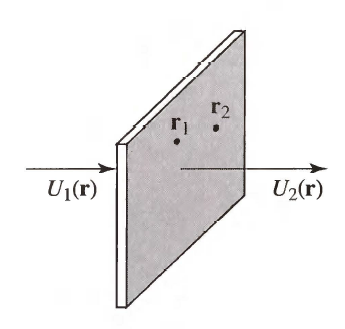
\includegraphics[width=0.3\textwidth]{11_3_1.PNG}
\caption{通过一个薄光学元件并不会改变空间相干度的绝对值。}
\label{fig: 11_3_1}
\end{figure}
\par 位置$r$处的光强等于互强度在$r_1 =  r_2 = r $时的值
\begin{equation}
I_2 (r) = \lvert t(r) \rvert ^2 I_1 (r) .
\end{equation}
故由(11.1-27)定义的归一化的互强度满足
\begin{equation}
\lvert g_2 (r_1, r_2) \rvert = \lvert g_1 (r_1, r_2) \rvert .
\end{equation}
尽管通过薄光学元件可能会改变部分相干光的光强,但并不会改变部分相干光的空间相干度的模。自然,若复振幅透过率自身是随机的,则透射光的相干性也会改变。
\bigbreak\noindent\textcolor{ksc}{\textbf{\textsl{通过任意光学系统的传播}}}\\
接下来,我们考察光在通过任意光学系统的传播,其涵盖了光在自由空间中传播和光通过薄光学元件传播的情况。我们在第四章看到,任意光学系统输出平面上点 $r = (x,y)$处的复振幅$U_2 (r)$,都可以看成是,输入平面上点$r' = (x', y')$处的复振幅$U_1 (r')$的贡献的加权积分 (见 图 11.3-2),
\begin{equation}
U_2 (r) = \int h(r; r') U_1 (r') \dif r' ,
\end{equation}
其中,$h(r, r')$为光学系统的脉冲响应函数。(11.3-4)中二重积分的积分变量 $r' = (x', y')$的范围是整个输入平面。
\begin{figure}[H]
\centering
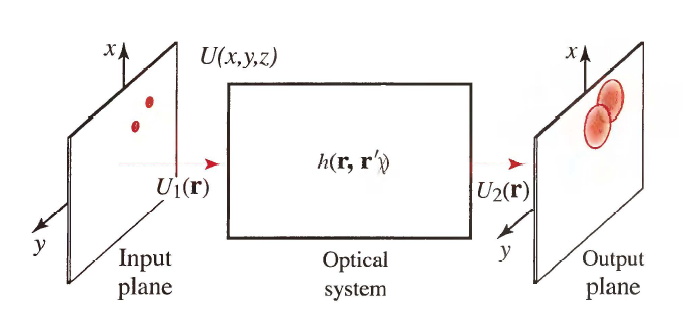
\includegraphics[width=0.7\textwidth]{11_3_2.PNG}
\caption{An optical system is characterized by its impulse response function $h(r; r')$.}
\label{fig: 11_3_2}
\end{figure}
\par 为了将随机函数$U_2 (r)$与 $U_1 (r')$的关系转化为其互强度之间的关系,我们将(11.3-4)代入定义 $G_2 (r_1, r_2) = \langle U_2^\ast (r_1) U_2(r_2) \rangle$,并利用定义$G_1(r'_1, r'_2) = \langle U_1^\ast (r'_1) U_1(r'_2) \rangle$可得
\begin{equation}
G_2 (r_1, r_2) = \iint h^\ast (r_1; r'_1) h(r_2; r'_2) G_1 (r'_1, r'_2) \dif r'_1 \dif r'_2 .
\end{equation}
\par 我们可以利用定义 $I_2 (r) = G_2 (r, r)$退化等式(11.3-5),获得输出光的光强
\begin{equation}
I_2 (r) = \iint h^\ast (r; r'_1) h(r; r'_2) G_1 (r'_1, r'_2) \dif r'_1 \dif r'_2 .
\end{equation}
因此,为了确定输出光的光强$I_2 (r)$,仅有输入光的光强$I_1 (r')$是不够的,我们必须知道输入光的互强度。
\bigbreak\begingroup
\color{ksc}
\subsubsection{非相干光成像}
\endgroup
现在,我们考虑输入光是非相干光的特殊情况。此时,只要$r'_2$稍微偏离$r'_1$一点,互强度$G_1 (r'_1, r'_2)$就等于0,故相干距离比系统中的其他相关尺寸(譬如成像系统的分辨率)要小得多。互强度可以写成$G_1 (r'_1, r'_2) = \sqrt{I_1 (r'_1) I_1(r'_2)} g(r'_1 - r'_2)$的形式,其中,$g(r'_1 - r'_2)$为一窄宽函数。当$G_1 (r'_1, r'_2)$出现在(11.3-5) 或 (11.3-6)的积分号下时,为了方便,可以用一个$\delta$函数带代替 $g(r'_1 - r'_2)$,即令$g(r'_1 - r'_2) = \sigma \delta (r'_1 - r'_2)$,其中,  $\sigma = \int g(r') \dif r'$为$g(r')$下的面积。故我们可得
\begin{equation}
G_1 (r'_1, r'_2) \approx \sigma \sqrt{I_1 (r'_1) I_1 (r'_2)} \delta (r'_1 - r'_2) .
\end{equation}
因为互强度的值一定是有限的而 $\delta (0) \to \infty$,所以上式显然不在普遍意义上正确,而只在计算形如 (11.3-6)中的积分时有效。将(11.3-7)代入 (11.3-6),$\delta$函数化简了二重积分,我们可得
\begin{equation}
I_2 (r) = \int I_1 (r') h_i (r; r') \dif r' ,
\end{equation}
其中
\begin{equation}
h_i (r; r') = \sigma \lvert h(r; r') \rvert ^2 .
\end{equation}
\par 在这些条件下,输入平面的光强与输出平面的光强之间的关系,描述了一个脉冲响应函数(也称为\textbf{点扩散函数})为$h_i (r; r')$的线性系统。因此,当输入光是完全非相干的,输出平面上任意一点$r$的光强就等于输入平面上所有点$r'$的光强的贡献的加权积分。并没有干涉发生,光强只是简单地相加(图 11.3-3)。与此形成对比的是,对于完全相干系统而言,进行加权积分的是复振幅而不是光强(见(11.3-4))。
\begin{figure}[H]
\centering
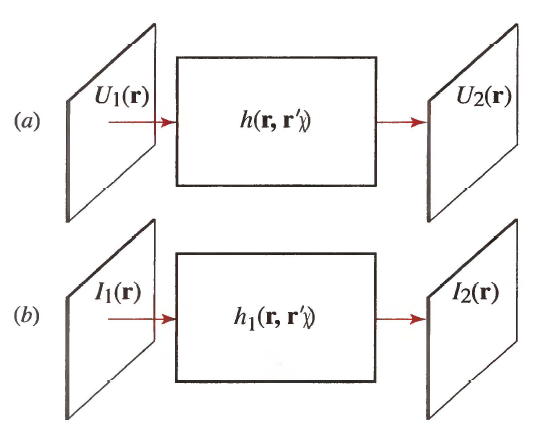
\includegraphics[width=0.5\textwidth]{11_3_3.PNG}
\caption{(a) 对于照明光为相干光的光学系统,输入平面的复振幅经过一脉冲响应函数为$h(r; r')$的线性系统得到输出平面的复振幅。(b)对于照明光为非相干光的光学系统,输入平面的光强经过一脉冲响应函数为$h_i (r; r') = \sigma \lvert h(r; r') \rvert ^2$的线性系统得到输出平面的光强。}
\label{fig: 11_3_3}
\end{figure}
\par 在某些光学系统中,脉冲响应函数是 $r-r'$的函数,记为$h(r - r')$。此时,我们称系统是移不变的或等晕的(见 Appendix B)。(11.3-4) 和(11.3-8)中的积分便均可化为二维的卷积,且相干系统和非相干系统可分别用I$h(r) = h(x,y)$的傅里叶变换$H(\nu_x, \nu_y)$ 和$h_i (r) = h_i (x,y)$的傅里叶变换 $H_i(\nu_x, \nu_y)$来描述,其中,$H(\nu_x, \nu_y)$和 $H_i(\nu_x, \nu_y)$均称为传递函数。
\par 举个例子,我们将两个点扩散函数的关系应用到单透镜成像系统中。 我们在 Sec. 4.4C 中看到,相干光照明时,如图 11.3-4所示的单透镜成像系统的脉冲响应函数,在 Fresnel近似条件下为
\begin{equation}
h(r) \propto P(\frac{x}{\lambda d_2}, \frac{y}{\lambda d_2}) ,
\end{equation}
其中,$P(\nu_x, \nu_y)$ 为光瞳函数$p(x, y)$的傅里叶变换,$d_2$为像面到透镜的距离。光瞳函数在光阑内等于1,在其余处等于0。
\par 当照明光是准单色的且空间非相干时,物平面的的光强和像平面的光强可以用一脉冲响应函数为
\begin{equation}
h_i (r) = \sigma \lvert h(r) \rvert ^2 \propto \lvert P(\frac{x}{\lambda d_2}, \frac{y}{\lambda d_2}) \rvert ^2 ,
\end{equation}
的系统线性关联起来,其中,$\lambda$ 为中心频率$\nu_0$对应的波长。\\
\begin{figure}[H]
\centering
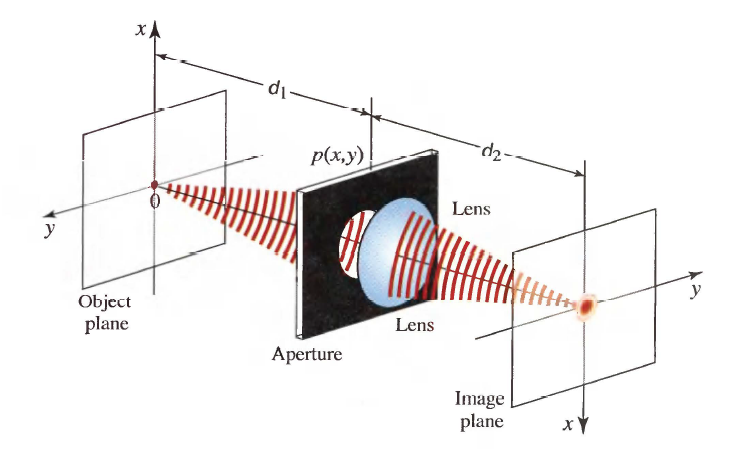
\includegraphics[width=0.7\textwidth]{11_3_4.PNG}
\caption{单透镜成像系统}
\label{fig: 11_3_4}
\end{figure}
\noindent{\crule[ksc]{\textwidth}{0.1cm}}
\textbf{EXAMPLE 11.3-1.具有圆形光阑的成像系统.} 若光阑是半径为 $a$的圆,则光瞳函数对于圆内的$x,y$有$p(x,y) = 1$,在其余处等于0。光瞳函数的傅里叶变换为
\begin{equation}
P(\nu_x, \nu_y) = \frac{a J_1 (2\pi \nu_\rho a)}{\nu_\rho} , \quad \nu_\rho = \sqrt{\nu_x^2 + \nu_y^2} ,
\end{equation}
其中$J(\cdot)$ 是贝塞尔函数(见 Appendix A, Sec. A.3). 代入上式到(11.1-36)中,可得相干照明下的脉冲响应函数
\begin{equation}
h(x,y) \propto [\frac{J_1 (2\pi\nu_s \rho)}{\pi\nu_s \rho}] , \quad \rho = \sqrt{x^2 + y^2} ,
\end{equation}
其中
\begin{equation}
\nu_s = \frac{\theta}{2 \lambda} , \quad \theta = \frac{2a}{d_2} .
\end{equation}
因此,非相干照明下的脉冲响应函数为
\begin{equation}
h_i (x,y) \propto [\frac{J_1 (2\pi\nu_s \rho)}{\pi\nu_s \rho}]^2 .
\end{equation}
\par 图 11.3-5画出了脉冲响应函数$h(x,y)$和$h_i (x,y)$。两个函数都在$2\pi \nu_s \rho = 3.832$时,即 $\rho = \rho_s \approx 3.832 / 2\pi \nu_s = 3.832\lambda / \pi\theta$时到达第一个零点。 代入$\pi$的值可得
\begin{equation}
\rho_s \approx 1.22 \frac{\lambda}{\theta} .
\end{equation}
因此,输入平面上的一个点(脉冲)成的像是一光强为$h (x,y)$或$h_i (x,y)$,半径为$\rho_s$的斑。当输入是由两个相距为$\rho_s$的两个点(脉冲)构成时,其中一个点成的像消失于另一个点成的像的中心。故距离 $\rho_s$是成像系统分辨率的一个测度。
\begin{figure}[H]
\centering
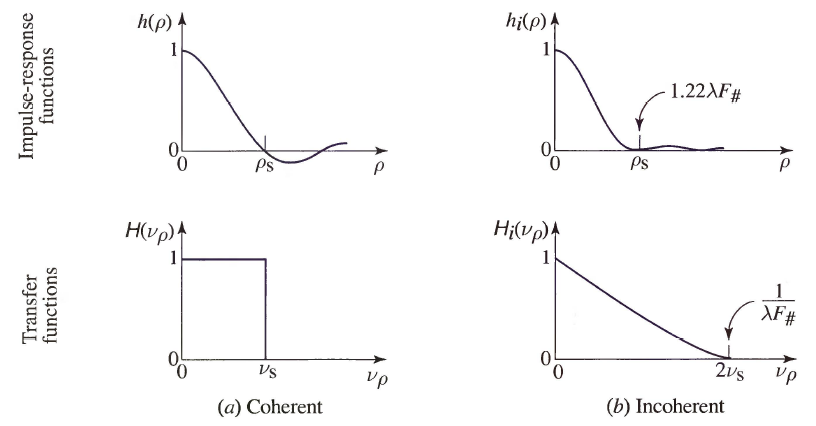
\includegraphics[width=0.9\textwidth]{11_3_5.PNG}
\caption{在(a)相干照明  和 (b)非相干照明 情况下,具有圆形光阑,F数为$F_\#$的单透镜衍射受限成像系统的脉冲响应函数和传递函数。}
\label{fig: 11_3_5}
\end{figure}
\par 具有上述脉冲响应函数$h(x,y)$或 $h_i (x,y)$的线性移不变系统(见 Appendix B)的传递函数,分别为其脉冲响应函数的傅里叶变换(见 Appendix A)
\begin{equation}
H(\nu_x, \nu_y) =
\begin{cases}
1, & \nu_\rho < \nu_s \\
0, & otherwise,
\end{cases}
\end{equation}
和
\begin{equation}
H_i (\nu_x, \nu_y) =
\begin{cases}
\frac{2}{\pi} \Big[\cos^{-1} \frac{\nu_\rho}{2\nu_s} -  \frac{\nu_\rho}{2\nu_s} \sqrt{1 - ( \frac{\nu_\rho}{2\nu_s})^2} \Big], & \nu_\rho < 2\nu_s \\
0, & otherwise,
\end{cases}
\end{equation}
其中 ,$\nu_\rho = \sqrt{v_x^2 + v_y^2}$。 两个函数均已归一化使得$\nu_\rho = 0$ 时其值为0。这些函数都画于图 11.3-5中。对于相干光照明,传递函数是平的且截至频率$\nu_s = \theta / 2 \lambda$线对/mm。对于非相干光照明,传递函数随着空间频率的增加近似线性下降,截至频率为$2\nu_s = \theta / \lambda$线对/mm。
\par 若物体放置于无穷远,即$d_1 = \infty$,则像在透镜焦距处,即$d_2 = f$。此时, 角度$\theta$ 等于$2a / f$,刚好为透镜的F数$F_\# = f / 2a$的倒数。截止频率 $\nu_s$和 $2\nu_s$可分别用F数表示
\begin{equation}
\text{截止频率(线对/mm)} =
\begin{cases}
\frac{1}{2 \lambda F_\#} & (\text{相干照明}) \\
\frac{1}{\lambda F_\#} & (\text{非相干照明}) .
\end{cases}
\end{equation}
\par 你可能会下这样一个错误的结论:非相干照明比相干照明更优越,缘于其空间带宽是相干照明的两倍。然而,我们不应该直接比较两个照明下的传递函数,因为相干照明下的传递函数描述的是复振幅的成像,而非相干照明下的传递函数描述的是光强的成像。\\
\noindent{\crule[ksc]{\textwidth}{0.1cm}}

\bigbreak\begingroup
\color{ksc}
\subsubsection{通过传播获得空间相干性}
\endgroup
等式(11.3-5)描述了光通过脉冲响应函数为$h(r; r')$的光学系统后互强度的变化。当输入光是非相干光时,(11.3-5)中的$G_1 (r'_1, r'_2)$可以用$\sigma \sqrt{I_1 (r'_1) I_1 (r'_2)} \delta (r'_1 - r'_2)$代替,积分化简为
\begin{equation}
G_2 (r_1, r_2) = \sigma \int h^\ast (r_1; r) h(r_2; r) I_1 (r) \dif r .
\end{equation}
\par 显然,输出光不再是非相干的。一般地,光通过单纯地传播行为就可以获得空间相干性。这没什么好惊讶的。尽管光在输入平面上各点的涨落是不相关的,但是各点的辐射在传播的过程中与相邻点的辐射发生重叠。到达输出平面上两点的光来自于输入平面上的若干点,其中一部分点是相同的(见 图 11.3-6)。这些相同的点的贡献,使得输出平面上两点的涨落存在部分相关的关系。
\par 这个过程与非相关时间信号(白噪声)通过一个低通滤波器并没有什么不同。低通滤波器平滑了信号、减小了信号的频谱宽度,因此信号的相干时间变长,不再非相关。光在光学系统中的传播具有空间滤波器的作用,其减小了光的空间带宽,从而增大了光的相干面积。
\begin{figure}[H]
\centering
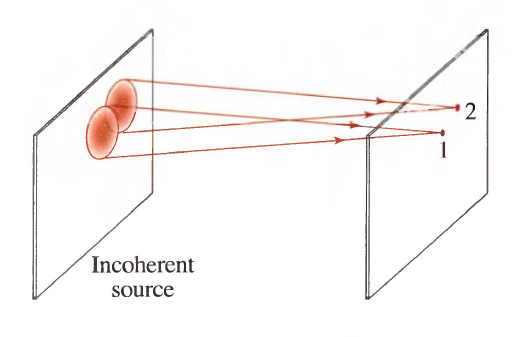
\includegraphics[width=0.5\textwidth]{11_3_6.PNG}
\caption{空间相干性的获得是光传播的结果。尽管光在光源处是完全空间非相关的,但是光在点1和点2处的涨落有相同的贡献源——阴影区域,因此两点处的涨落是部分空间相关的。}
\label{fig: 11_3_6}
\end{figure}
\bigbreak\noindent\textcolor{ksc}{\textbf{\textsl{Van Cittert-Zernike 定理}}}\\
在同一个光学系统中,空间非相干光缘于传播的空间相干性的获得,与相干光复振幅的改变存在数学上的相似性。参考 (11.3-20),若观察点$r_1$固定,譬如说在原点,则互强度$G_2 (0, r_2)$是 $r_2$的函数
\begin{equation}
G_2(0, r_2) = \sigma \int h^\ast (0; r) h(r_2; r) I_1 (r) \dif r .
\end{equation}
定义 $U_2 (r_2) = G_2 (0, r_2)$ , $U_1 (r) = \sigma h^\ast (0; r) I_1 (r)$, 则 (11.3-21) 可以写成我们熟悉的形式
\begin{equation}
U_2(r_2) = \int h(r_2; r) U_1 (r) \dif r ,
\end{equation}
这正是约束相干光传播的积分(11.3-4)。因此,在同一个光学系统中,非相干照明下输出平面上的互强度 $G(0, r_2)$,在数学上等价于相干光照明下,输入光的复振幅为$U_1 (r) = \sigma h^\ast (0; r) I_1 (r)$时,输出平面上的复振幅。 
\par 举个例子,假设非相干输入光均匀遍布在光阑$p(r)$上(光阑内$p(r) = 1$,其余处为0),即$I_1 (r) = p(r)$,并假设光学系统是自由空间,即$h(r'; r) = \exp (-jk\lvert r' - r \rvert) / \lvert r' - r \rvert$,则若要相干照明时的复振幅$U_2 (r_2)$与非相干照明时的互强度$G_2 (0, r_2)$相同,相干照明时输入光的复振幅必须为$U_1 (r) = \sigma h^\ast (0; r) p(r) = \sigma p(r) \exp (jkr) / r$。此时,输入光为通过光阑的、收敛到输出平面上原点的球面波。
\par 空间非相干光缘于传播的空间相干性的获得,与相干光复振幅的改变之间的数学上的相似性称为\textbf{Van Cittert-Zernike 定理}。
\bigbreak\noindent\textcolor{ksc}{\textbf{\textsl{自由空间中相干性的获得}}}\\
考虑一由两相距为$d$的平行平面间的自由空间构成的光学系统(图 11.3-7),其输入平面上的光是准单色的、空间非相干的,且强度$I(x,y)$在有限区域内延伸。距离 $d$足够大,以致对于输出平面上感兴趣的点Fraunhofer近似都是有效的。在这些条件下,我们可以用Fraunhofer衍射公式[见 (4.2-3)]来描述光学系统
\begin{equation}
h(r; r') = h_0 \exp (-j\pi \frac{x^2 + y^2}{\lambda d}) \exp (j2\pi \frac{xx' + yy'}{\lambda d}),
\end{equation}
其中, $r = (x,y,d)$ ,$r' = (x', y', 0)$ 分别是输出平面和输入平面上的点,$h_0 = (j / \lambda d) \exp(-j2\pi d / \lambda)$为一常数。
\begin{figure}[H]
\centering
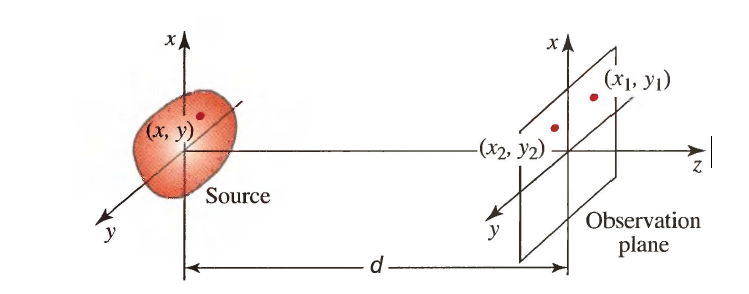
\includegraphics[width=0.8\textwidth]{11_3_7.PNG}
\caption{自由空间中空间非相干光源的辐射。}
\label{fig: 11_3_7}
\end{figure}
\par 为了确定输出平面上点$(x_1, y_1)$与点$(x_2, y_2)$ 处的互强度$G(x_1, y_1, x_2, y_2)$ ,我们将(11.3-23)代入(11.3-20) ,得 
\begin{equation}
\lvert G(x_1, y_1, x_2, y_2) \rvert = \sigma_1 \bigg\lvert \iint\limits_{-\infty}^{+\infty} \exp \{j\frac{2\pi}{\lambda d} [(x_2 - x_1)x + (y_2 - y_1)y]\}I(x,y) \dif x \dif y \bigg\rvert ,
\end{equation}
其中, $\sigma_1 = \sigma \lvert h_0 \rvert ^2 = \sigma / \lambda ^2 d^2$为常数。不难看出,若已知输入平面上的光强$I(x,y)$,则我们可以通过计算$I(x,y)$的二维傅里叶变换
\begin{equation}
\mathcal{J} = \iint\limits_{-\infty}^{+\infty}\exp [j2\pi (\nu_x x+ \nu_y y)] I(x,y) \dif x \dif y
\end{equation}
在$\nu_x = (x_2 - x_1) / \lambda d$ ,$\nu_y = (y_2 - y_1) / \lambda d$处的值轻松得到输出平面上的互强度的模$\lvert G(x_1, y_1, x_2, y_2) \rvert$。归一化得
\begin{equation}
\lvert g(x_1, y_1, x_2, y_2) \rvert = \bigg\lvert \mathcal{J}(\frac{x_2 - x_1}{\lambda d}, \frac{y_2 - y_1}{\lambda d}) \bigg\rvert / \mathcal{J}(0, 0) .
\end{equation}
非相干光源的光强与其远场空间相干度之间的这种傅里叶变换关系,与相干光的复振幅与其远场复振幅之间的傅里叶变换关系(见 Sec. 4.2A)非常相似。这种相似性是蕴含于 Van Cittert-Zernike 定理之中的。
\par (11.3-26)的意义深远。该式表明,输入平面上的光源的面积(即$I(x,y)$的空间尺度)越小,则其傅里叶变换 $\mathcal{J}(\nu_x, \nu_y)$就越宽,因此输出平面上的互强度延伸的面积就越大,相干面积就越大。在一个极限情况下,输入平面上的光都在一个点上,此时的相干面积无穷大且辐射场也是完全空间相干的。这个结论证实了我们前面在Sec. 11.1 D中关于球面波空间相干性的讨论。另一方面,若输入平面的非相干光源为一个大的扩展光源,则输出平面上的相干面积就小。\\
\noindent{\crule[ksc]{\textwidth}{0.1cm}}
\textbf{EXAMPLE 11.3-2. 空间非相干圆形光源的辐射.} 若输入光的光强为$I(x,y) = I_0$且受限于半径为a的圆形光阑,则(11.3-26)可得
\begin{equation}
\lvert g(x_1, y_1, x_2, y_2) \rvert = \bigg\lvert \frac{2J_1(\pi\rho\theta_s / \lambda)}{\pi\rho\theta_s / \lambda} \bigg\rvert ,
\end{equation}
其中, $\rho = \sqrt{(x_2 - x_1)^2 + (y_2 - y_1)^2}$ 为两点间的距离, $\theta_s = 2a / d$ 为光源的张角, $J_1 (\cdot)$为Bessel 函数。这些几何参数都画在了图 11.3-8中。Bessel 函数在其参数为$3.832$时到达第一个零点,故我们可以定义相干距离(相干面积为半径为相干距离的圆的面积) $\rho_c = 3.832(\lambda / \pi\theta_s)$, 即
\begin{equation}
\rho_c = 1.22 \frac{\lambda}{\theta_s} .
\end{equation}
我们曾在前面使用不太严格的分析得到类似的结果(11.2-18)。显然相干面积反比于$\theta_s^2$。举个例子,当非空间相干光源的波长 $\lambda = 0.6 \mu$m,半径为$1$cm时,其在距离$d = 100$m的观察平面上的相干距离$\rho_c \approx 3.7$mm。
\begin{figure}[H]
\centering
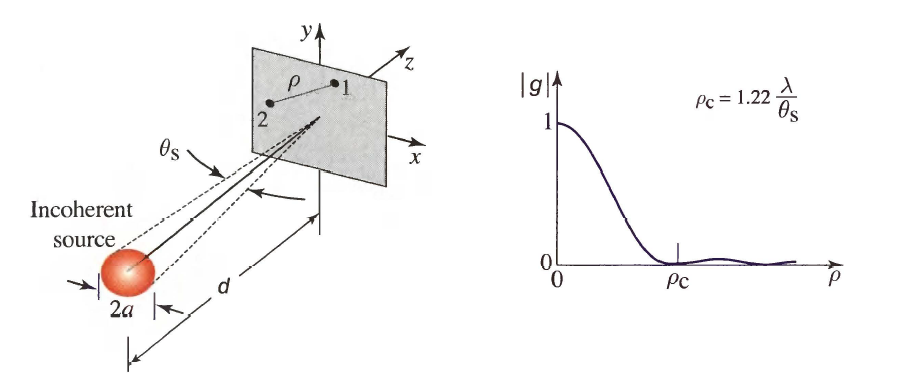
\includegraphics[width=0.8\textwidth]{11_3_8.PNG}
\caption{由张角为 $\theta_s$的空间非相干圆形光源发出的光的空间相干度的模,其为一距离$\rho$的函数。}
\label{fig: 11_3_8}
\end{figure}
\noindent{\crule[ksc]{\textwidth}{0.1cm}}
\bigbreak\noindent\textcolor{ksc}{\textbf{\textsl{测量恒星的角直径:Michelson恒星干涉仪}}}\\
等式(11.3-28)是测量恒星角直径的方法基础。若将恒星视作一直径为$2a$,亮度均匀的圆盘,则当距离恒星$d$处的观察平面上的两点间距为$\rho_c = 1.22 \lambda / \theta_s$时,互强度降至0。在一给定的波长$\lambda$ 下测量 $\rho_c$,就能确定角直径$\theta_s = 2a / d$。
\par 举个例子,取太阳的角直径为$0.5\degree$,即$\theta_s = 8.7 \times 10^{-3}$弧度,并假设光强是均匀的,我们有 $\rho_c = 140\lambda$。当$\lambda = 0.5 \mu$m时,$\rho_c = 70 \mu$m。 For $\lambda = 0.5 \mu$m, $\rho_c = 70 \mu$m. 故此时若要在杨氏双缝干涉仪中观察到干涉条纹,双缝间距必须小于70 $\mu$m。恒星的角直径越小,其相干面积就越大。譬如,第一颗使用此技术测量角直径的恒星($\alpha\text{-Orion}$)的角直径为$\theta_s = 22.6\times 10^{-8}$,故$\lambda = 0.57 \mu$m时,$\rho_c = 3.1$m。如图11.3-9所示,我们可以通过在杨氏双缝干涉仪中加入可移动的镜子来扩展其可用缝间距,使其可测相距$3.1$m的两点的互强度。
\begin{figure}[H]
\centering
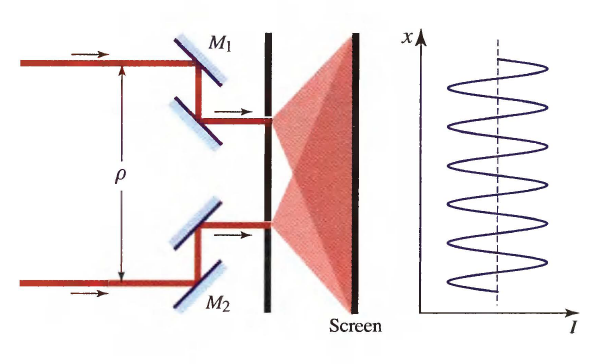
\includegraphics[width=0.5\textwidth]{11_3_9.PNG}
\caption{Michelson恒星干涉仪。我们通过使用杨氏双缝干涉仪测量相距$\rho$的两点的互强度,来估计恒星的角直径。我们不断改变镜子$M_1$与$M_2$之间的距离,同时测量干涉条纹的可见度。当  $\rho = \rho_c = 1.22\lambda / \theta_s$时,可见度等于0。}
\label{fig: 11_3_9}
\end{figure}

\bigbreak\begingroup
\color{ksc}
\subsection{部分偏振}
\endgroup
正如我们在第六章所看到的,光的标量理论通常不够准确,因此考虑了光的偏振的矢量理论是必要的。本节简单讨论考虑了偏振作用的随机光的统计理论。\textbf{部分偏振理论}是建立在以相关与互相关(与本章前面的定义相似)描述光场的矢量成分的基础上的。
\par 为了简化表述,我们不会考虑空间效应,因此我们只讨论光是沿z轴方向传播的横向电磁(transverse electrimagnetic, TEM)平面波的情形。此时,光的电矢量只有$x$方向的和 $y$方向的两个分量,其随机复振幅分别为$U_x (t)$、$U_y (t)$。我们用自相关函数(时间相干函数)来描述每个方向的分量,
\begin{align}
G_{xx}(\tau) &= \langle U_x^\ast (t) U_x(t + \tau) \rangle \\
G_{yy}(\tau) &= \langle U_y^\ast (t) U_y(t + \tau) \rangle .
\end{align}
另外一个随机偏振波的描述量是 $U_x (t)$ 与 $U_y (t)$的互相关函数
\begin{equation}
G_{xy}(\tau) = \langle U_x^\ast (t) U_y(t + \tau) \rangle .
\end{equation}
归一化后的函数为
\begin{equation}
g_{xy} = \frac{G_{xy}(\tau)}{\sqrt{G_{xx}(0)G_{yy}(0)}}
\end{equation}
即为$U_x (t)$ 与$U_y(t + \tau)$的互相关系数。其满足不等式 $0 \le \vert g_{xy}(\tau) \rvert \le 1$。若两分量在任意时刻都不相关,则$\lvert g_{xy}(\tau) \rvert = 0$;若两分量在任意时刻都完全相关,则$\lvert g_{xy}(\tau) \rvert = 1$。
\par 一般地,频谱特性与偏振特性有关,且自相关函数和互相关函数对时间延迟$\tau$的依赖可以不同。但对于准单色光,(11.4-1) 到(11.4-4)中,函数对$\tau$的依赖关系都近似具有$\exp (j\omega_0 \tau)$的形式。因此,我们可以用函数在 $\tau = 0$处的值,即$G_{xx}(0), G_{yy}(0)$和$G_{xy}(0)$(简记为$G_{xx}, G_{yy}$, $G_{xy}$),来描述偏振特性。注意,$G_{xx} = I_x$ 、$G_{yy} = I_y$都是实数,分别代表 $x$和 $y$方向的光强分量,而$G_{xy}$是复数,且根据其定义易得$G_{yx} = G_{xy}^\ast$。
\bigbreak\noindent\textcolor{ksc}{\textbf{\textsl{相干矩阵}}}\\
将四个数$G_{xx}, G_{xy}, G_{yx}$和 $G_{yy}$写成$2 \times 2$的HermitianI矩阵的形式很有用
\begin{equation}
\mathbf{G} = 
\begin{bmatrix}
G_{xx} & G_{xy} \\
G_{yx} & G_{yy}
\end{bmatrix}
\end{equation}
该矩阵称为\textbf{相干矩阵}。相干矩阵的主对角元素为光强$I_x$、$I_y$,副对角元素为互相关,迹 $Tr\mathbf{G} = I_x + I_y  \equiv \bar{I}$为总光强。
\par 相干矩阵也可以写成Jones向量$\mathbf{J} = \begin{bmatrix}U_x \\ U_y \end{bmatrix}$的形式,这里的Jones向量是用复波函数和复振幅定义的( Sec. 6.1B中的Jones向量是用复包络定义的)。
\begin{equation}
\langle \mathbf{J}^\ast \mathbf{J}^{\dag} \rangle = \langle 
\begin{bmatrix}
U_x^\ast \\
U_y^\ast
\end{bmatrix}
\begin{bmatrix}
U_x & U_y
\end{bmatrix}
\rangle =
\begin{bmatrix}
\langle U_x^\ast U_x \rangle & \langle U_x^\ast U_y \rangle \\
\langle U_y^\ast U_x \rangle & \langle U_y^\ast U_y \rangle 
\end{bmatrix}
= \mathbf{G} ,
\end{equation}
其中$\dag$表示矩阵的转置,$U_x$和$U_y$分别代表$U_x (t)$、$U_y (t)$。
\par 偏振装置,譬如偏振片和波片,会按照$\mathbf{J' = TJ}$ [见 (6.1-17)]的规则对Jones向量进行变换。其中, $\mathbf{T}$是代表装置的Jones矩阵 [见 (6.1-18) 到 (6.1-25)]。因此,相干矩阵经变换后变为$\mathbf{ G' = \langle T^\ast J^\ast (TJ)^\dag \rangle }$ $\mathbf{= \langle T^\ast J^\ast J^\dag R^\dag \rangle} $ $\mathbf{= T^\ast \langle J^\ast J^\dag \rangle T^\dag}$, 即
\begin{equation}
\mathbf{G' = T^\ast G T^\dag} .
\end{equation}
此即为偏振装置对部分偏振光的相干矩阵的影响的数学形式。
\bigbreak\noindent\textcolor{ksc}{\textbf{\textsl{Stokes参数和Poincar\'{e}球表示法}}}\\
我们在Sec. 6.1A中定义相干光的Stokes参数为4个与复包络的x分量和y分量乘积相关的实数[见 (6.1-9)]。这里我们将Stokes参数的定义对部分相干光进行广义化:
\begin{subequations}
\begin{alignat}{3}
S_0 &= \langle \lvert U_x \rvert^2 \rangle + \langle \lvert U_y \rvert^2 \rangle &=& G_{xx} + G_{yy} \\
S_1 &= \langle \lvert U_x \rvert^2 \rangle - \langle \lvert U_y \rvert^2 \rangle &= &G_{xx} - G_{yy} \\
S_2 &= 2Re\{\langle U_x^\ast U_y \rangle \} &=& 2Re\{G_{xy} \} \\
S_3 &= 2Im\{\langle U_x^\ast U_y \rangle \} &= &2Im\{G_{xy} \} .
\end{alignat}
\end{subequations} 
Stokes参数与相干矩阵$\mathbf{G}$的元素直接相关。第一个参数$S_0$就是相干矩阵的主对角元素和,即总光强$\bar{I}$。第二个参数$S_1$是相干矩阵的主对角元素差,即两个偏振分量的光强差。第三参数$S_2$和第四个参数$S_3$分别正比于相干矩阵的副对角元素,即互相关函数,的实部和虚部。利用这些关系式,我们可以由不等式$\lvert G_{xy} \rvert^2 \leq G_{xx}G_{yy}$推得不等式$S_1^2 + S_2^2 + S_3^2 \leq S_0^2$。对于相干光而言,这两个不等式退化为等式。
\par 部分偏振光的偏振状态在几何上可以用Poincar\'{e}球上一个笛卡尔坐标为($S_1 / S_0, S_2 / S_0, S_3 / S_0$)的点表示。因为 $S_1^2 + S_2^2 + S_3^2 \leq S_0^2$总是成立,故该点或者在球内,或者在球面上。
\par 为了理解相干矩阵和Stokes参数的重要性,接下来我们会考察两个极限的情形。
\bigbreak\noindent\textcolor{ksc}{\textbf{\textsl{非偏振光}}}\\
若光强为$\bar{I}$的光的两个方向的分量强度相同且不相关,即$I_x = I_y \equiv \frac{1}{2}\bar{I}$,$G_{xy} = 0$,则我们称该光是 \textbf{非偏振的}。此时,相干矩阵为
\begin{equation}
\mathbf{G} = \frac{1}{2}\bar{I}
\begin{bmatrix}
1 & 0 \\
0 & 1
\end{bmatrix}
\end{equation}
利用(11.4-7)和(6.1-22),我们可以证明, (11.4-9) 对坐标系统的旋转具有不变性,故非偏振光在任意两个正交方向的分量都是等强度且不相关的。故非偏振光的光场向量是统计各向同性的,即其等可能地分布在 $x-y$平面的所有方向上(图 11.4-1(a))。
\begin{figure}[H]
\centering
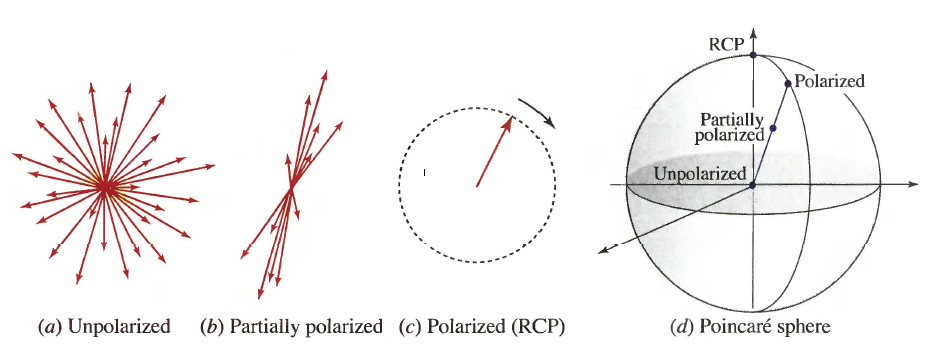
\includegraphics[width=0.9\textwidth]{11_4_1.PNG}
\caption{(a)非偏振、 (b) 部分偏振、 (c) 圆偏振的偏振(right circular polarization, RCP)光的电场向量的涨落;(d) Poincar\'{e} 表示法。}
\label{fig: 11_4_1}
\end{figure}
\par 非偏振光通过偏振片后变成线偏振光,但其仍然保持随机性且平均光强为 $\frac{1}{2}\bar{I}$。由于非偏振光的两个分量的相位本身就是随机的,而波片只是在两个分量间引入了一个相位差,故波片对非偏振光不起作用。类似地,非偏振光通过偏振旋转器仍然是非偏振光。偏振装置对光的这些作用都可以利用(11.4-7) 、(11.4.9) 与(6.1-18)、 (6.2-14)、(6.1-20)正式地表达出来。
\par 利用(11.4-8)和(11.4-9),我们随手就可以证明代表非偏振光的Stokes参数为$(S_0, S_1, S_2, S_3) = (\bar{I}, 0, 0, 0)$。其对应于Poincar\'{e}球上笛卡尔坐标为$(S_1 / S_0, S_2 / S_0, S_3 / S_0) = (0, 0, 0)$的一个点,即Poincar\'{e}球的球心。
\bigbreak\noindent\textcolor{ksc}{\textbf{\textsl{偏振光}}}\\
若互相关系数$g_{xy} = G_{xy} / \sqrt{I_x I_y}$的模为1,即$\lvert g_{xy} \rvert = 1$,则光场的两个分量是完全相关的,我们称该光是完全偏振的(或简单称为\textbf{偏振的})。此时,相干矩阵的形式为
\begin{equation}
\mathbf{G} = 
\begin{bmatrix}
I_x & \sqrt{I_x I_y}e^{j\varphi} \\
\sqrt{I_x I_y}e^{-j\varphi} & I_y
\end{bmatrix} ,
\end{equation}
其中, $\varphi$ 为$g_{xy}$的幅角。定义$U_x = \sqrt{I_x}$,$U_y = \sqrt{I_y}e^{j\varphi}$,则
\begin{equation}
\mathbf{G} =
\begin{bmatrix}
U_x^\ast U_x & U_x^\ast U_y \\
U_y^\ast U_x & U_y^\ast U_y
\end{bmatrix}
= \mathbf{J^\ast J^\dag} ,
\end{equation}
其中$\mathbf{J} = \begin{bmatrix}U_x \\ U_y \end{bmatrix}$.。此时 $\mathbf{G}$与 相干光的相干矩阵形式相同。利用表6.1-1提供的Jones向量,我们可以确定不同偏振态的相干矩阵。举两个例子:
\begin{equation*}
\text{$x$方向线偏振} \quad \mathbf{G} = \bar{I}
\begin{bmatrix}
1 & 0 \\
0 & 0 
\end{bmatrix}
\quad \text{右圆偏振} \quad \mathbf{G} = \frac{1}{2}\bar{I}
\begin{bmatrix}
1 & j \\
-j & 1
\end{bmatrix}
\end{equation*}
\par (11.4-11) 对应的Stokes参数满足关系式$S_1^2 + S_2^2 + S_3^2 = S_0^2$,故偏振光可用 Poincar\'{e}球的球面上(不在球内)的一个点表示。
\par 思考非偏振光与圆偏振光的区别是很有启发性的。对于非偏振光和圆偏振光,$x$方向的分量的强度都等于$y$方向上的分量的强度,即$(I_x = I_y)$。 非偏振光两分量是不相关的,而圆偏振光的两分量是完全相关的。非偏振光通过波片仍然是非偏振光,而圆偏振光通过波片后变为线偏振光。在Poincar\'{e}球表示法中,非偏振光位于球心,而圆偏振光位于南极点或北极点。
\bigbreak\noindent\textcolor{ksc}{\textbf{\textsl{偏振度}}}\\
部分偏振是随机光偏振的一般状态,这个状态介于非偏振和偏振之间。textbf{偏振度}的测度之一是用相干矩阵的行列式和迹定义的: 
\begin{align}
\mathbb{P} &= \sqrt{1 - \frac{4 det \mathbf{G}}{(Tr \mathbf{G})^2}} \\
&= \sqrt{1-4\frac{I_x I_y}{(I_x + I_y)^2}(1 - \lvert g_{xy} \rvert^2)} .
\end{align}
基于下面的考虑,这样定义的测度非常有意义
\par$\sqcdot$ 其满足不等式 $0 \leq \mathbb{P} \leq 1$.
\par$\sqcdot$ 对于偏振光,将 $\lvert g_{xy} = 1 \rvert$代入(11.4-13)可得$\mathbb{P}$取最大值1。对于非偏振光,由 $I_x = I_y$ and $g_{xy} = 0$可得$\mathbb{P} = 0$ 。
\par$\sqcdot$ 其对于坐标系统的旋转具有不变性(因为酉变换不改变矩阵的行列式和迹)。
\par$\sqcdot$ (11.4-13) 中的偏振度也可用Stokes参数表达:
\begin{equation}
\mathbb{P} = \frac{\sqrt{S_1^2 + S_2^2 + S_3^2}}{S_0} ,
\end{equation}
\par$\phantom{\sqcdot}$ 因此在 Poincar\'{e}球表示法中,其等于代表偏振态的点到球心的距离。
\par$\sqcdot$ 可以证明(Exercise 11.4-1),部分相干光总是可以看成是两个不相关的波的混合:其中一个是偏振光,另一个是非偏振光,偏振光的光强比上总光强等于$\mathbb{P}$。\\
\noindent{\crule[ksc]{\textwidth}{0.2cm}}
\textbf{EXERCISE 11.4-1} \\
\textbf{部分偏振光.} 证明当强度为$(I_x + I_y)(1 - \mathbb{P})$的非偏振光与强度为$(I_x + I_y)\mathbb{P}$的线偏振光发生叠加时,合成光的 $x$方向和$y$方向的光强分别为$I_x$ 与$I_y$,并求其归一化的互相关函数 $\lvert g_{xy} \rvert$。\\
\noindent{\crule[ksc]{\textwidth}{0.2cm}}

\clearpage
\pagestyle{empty}
\bigbreak\textcolor{ksc}{\huge{\textbf{\centerline{READING LIST}}}}\\
\begin{spacing}{0.5}
\bigbreak\noindent{\large\textbf{\textsl{General}}}\\
\begin{hangparas}{0.25cm}{1}
\par A. A. Kokhanovsky, Polarization Optics of Random Media, Springer-Verlag, 2003.\\
\par E. L. O'Neill, Introduction to Statistical Optics, Addison-Wesley, 1963; Dover, reissued 2003.\\
\par W. Lauterborn and T. Kurz, Coherent Optics: Fundamentals and Applications, Springer, 2nd ed.
2003.\\
\par M. Born and E. Wolf, Principles of Optics, Cambridge University Press, 7th expanded and corrected
ed. 2002, Chapter 10.\\
\par B. R. Frieden, Probability, Statistical Optics, and Data Testing: A Problem Solving Approach,
Springer-Verlag, 1983, 3rd ed. 2001.\\
\par J. W. Goodman, Statistical Optics, Wiley, 1985, paperback ed. 2000.\\
\par H. E. Rowe, Electromagnetic Propagation in Multi-Mode Random Media, Wiley, 1999.\\
\par C. Brosseau, Fundamentals of Polarized Light: A Statistical Optics Approach, Wiley, 1998.\\
\par L. Mandel and E. Wolf, Optical Coherence and Quantum Optics, Cambridge University Press, 1995.\\
\par H. Le£ 七vre, The Fiber-Optic Gyroscope, Artech, 1993.\\
\par G. Reynolds, J.B. De Velis, G. B. Parrent, and B. J. Thompson, The New Physical Optics Notebook:
\par Tutorials in Fourier Optics, SPIE Optical Engineering Press, 1989.\\
\par J. Perina, Coherence of Light, Reidel, 1971, 2nd ed. 1985.\\
\par J.C. Dainty, ed., Laser Speckle and Related Phenomena, Springer-Verlag, 1975, 2nd ed. 1984.\\
\par A. S. Marathay, Elements of Optical Coherence Theory, Wiley, 1982.\\
\par B. E. A. Saleh, Photoelectron Statistics with Applications to Spectroscopy and Optical Communication, Springer-Verlag, 1978.\\
\par B. Crosignani, P. Di Porto, and M. Bertolotti, Statistical Properties of Scattered Light, Academic
Press, 197 5.\\
\par M. J. Beran and G. B. Parrent, Jr., Theory of Partial Coherence, Prentice Hall, 1964; SPIE Optical
Engineering Press, reissued 1974.\\
\par R. Hanbury-Brown, The Intensity Interferometer: Its Application to Astronomy, Taylor \& Francis,
1974.\\
\par G. J. Troup, Optical Coherence Theory', Methuen, 1967.\\


\bigbreak\noindent{\large\textbf{\textsl{Books on Random Functions}}}\\
\par A. Papoulis and S. U. Pillai, Probability, Random Variables, and Stochastic Processes, McGraw-Hill,
1965, 4th ed. 2002.\\
\par E. Parzen, Stochastic Processes, Holden-Day, 1962; Society for Industrial and Applied Mathematics
(SIAM), reissued 1999.\\
\par E. Parzen, Modern Probability Theory and Its Applications, Wiley, 1960, paperback ed. 1992.\\
\par C. W. Helstrom, Probability and Stochastic Processes for Engineers and Scientists, Macmillan, 2nd.
ed. 1991.\\
\par W. B. Davenport, Jr., and W. L. Root, An Introduction to the Theory of Random Signals and Noise,
McGraw-Hill, 1958; IEEE Press, reissued 1987.\\
\par E. Vanmarcke, Random Fields, MIT Press, 1983.\\
\par J.B. Thomas, An Introduction to Applied Probability and Random Processes, Wiley, 1971.\\


\bigbreak\noindent{\large\textbf{\textsl{Books on Optical Coherence Tomography}}}\\
\par M. E. Brezinski, Optical Coherence Tomography: Principles and Applications, Academic Press,
2006.\\
\par W. Drexler, ed., Optical Coherence Tomography and Coherence Techniques, Volume 2, Progress in Biomedical Optics and Imaging, SPIE Optical Engineering Press, 2005.\\
\par W. Drexler, ed., Optical Coherence Tomography and Coherence Techniques, Volume 1, Progress in
Biomedical Optics and Imaging, SPIE Optical Engineering Press, 2003.\\
\par B. E. Bouma and G. J. Teamey, eds., Handbook of Optical Coherence Tomography, Marcel Dekker,
2002.\\


\bigbreak\noindent{\large\textbf{\textsl{Articles}}}\\
\par P. H. Tomlins and R. K. Wang, Theory, Developments and Applications of Optical Coherence Tomography,
\par Journal of Physics D: Applied Physics, vol. 38, pp. 2519—2535, 2005.\\
\par A. F. Fercher, W. Drexler, C. K. Hitzenberger, and T. Lasser, Optical Coherence Tomography—
Principles and Applications, Reports on Progress in Physics, vol. 66, pp. 239-303, 2003.\\
\par L. Mandel and E. Wolf, eds., Selected Papers on Coherence and Fluctuations of Light (1850-1966), SPIE Optical Engineering Press (Milestone Series Volume 19), 1990.\\
\par R. B. Smith, ed., Selected Papers on Fiber Optic Gyroscopes, SPIE Optical Engineering Press (Milestone Series Volume 8), 1989.\\
\par Feature issues on applications of coherence and statistical optics, Journal of the Optical Society of
America, no. 7, 1986 and no. 8, 1986.\\
\par F. T. S. Yu, Principles of Optical Processing with Partially Coherent Light, in Progress in Optics,
vol. 23, E. Wolf, ed., North-Holland, 1986.\\
\par W. J. Tango and R. Q. Twiss, Michelson Stellar Interferometry, in Progress in Optics, vol. 17, E. Wolf,
ed., North-Holland, 1980.\\
\par G. 0. Reynolds and J.B. De Velis, Review of Optical Coherence Effects in Instrument Design, SPIE
Proceedings, vol. l94, pp. 2-33, 1979.\\
\par H. P. Baltes, J. Geist, and A. Walther, Radiometry and Coherence, in Inverse Source Problems in
Optics, H. P. Baltes, ed., Springer-Verlag, 1978.\\
\par E. Wolf, Coherence and Radiometry, Journal of the Optical Society of America, vol. 68, pp. 6-17,
1978.\\
\par L. Mandel and E. Wolf, eds., Selected Papers on Coherence and Fluctuations of Light, Volumes .l
and 2, Dover, 1970.\\
\par B. J. Thompson, Image Formation with Partially Coherent Light, in Progress in Optics, vol. 7,
E. Wolf, ed., North-Holland, 1969.\\
\par L. Mandel and E. Wolf, Coherence Properties of Optical Fields, Reviews of Modem Physics, vol. 37,
pp.231-287, 1965.\\
\end{hangparas}
\end{spacing}

\bigbreak\textcolor{ksc}{\huge{\textbf{\centerline{PROBLEMS}}}}
\bigbreak
{
\setlength{\parskip}{2ex}
\begin{hangparas}{1.4cm}{1}
\par 11.1-4 \quad\textbf{Lorentzian 频谱.} 一发光二极管(LED)发出Lorentzian频谱的、带宽$\Delta\nu (FWHM) = 10^{13} Hz$、中心波长 $\lambda_0 = 0.7 \mu m$的光。试确定其线宽$\Delta\lambda_0$(单位nm)、相干时间$\tau_c$、相干时间 $l_c$。复时间相干度的模$\lvert g(\tau) \rvert$大于0.5时对应的最大时间延迟是多少?
\par 11.1-5 \quad\textbf{证明Wiener-Khinchin定理.} 利用(11.1-4)、 (11.1-14)、(11.1-15) 中的定义证明频谱密度 $S(\nu)$是自相关函数$G(\tau)$的傅里叶变换。证明光强 $I$ 是功率频谱密度$S(\nu)$.的积分。
\par 11.1-6 \quad\textbf{互强度.} 一光波在$x$轴上点的互强度为
\begin{equation*}
G(x_1, x_2) = I_0 \exp [- \frac{(x_1^2 + x_2^2)}{W_0^2}]\exp [- \frac{(x_1 - x_2)^2}{\rho_c^2}] ,
\end{equation*}
其中,$I_0, W_0$, $\rho_0$均为常数。试画出光强作为$x$的函数的草图。推导归一化互强度$g(x_1, x_2)$的表达式并画出其作为 $x_1 - x_2$的函数的草图。$I_0, W_0$, $\rho_c$的物理意义是什么?
\par 11.1-7 \quad\textbf{互相干函数.} 一光波在$x$轴上点的互相干函数为
\begin{equation*}
G(x_1, x_2, \tau) = \exp (- \frac{\pi \tau^2}{2 \tau_c^2})\exp [j2\pi \mu (x_1, x_2)\tau] \exp[- \frac{(x_1 - x_2)^2}{\rho_c^2}] ,
\end{equation*}
其中,$x_1 + x_2 > 0$时 $u(x_1, x_2) = 5 \times 10^{14} s^{-1}$,$x_1 + x_2 < 0$时$u(x_1, x_2) = 6 \times 10^{14} s^{-1}$,$\rho_c = 1 mm$, $\tau_c = 1\mu s$。试确定光强、功率频谱密度、相干长度和横向相干距离。这些量中的哪一个或哪些是位置独立的?如果这个光被记录在彩色胶卷上,图像看起来是什么样? 
\par 11.1-8 \quad\textbf{相干长度.} 证明窄带光的相干长度为$l_c \approx \lambda^2 / \Delta\lambda$,其中$\Delta\lambda$为线宽。证明频谱均匀分布在 $\lambda_{min}$与 $\lambda_{max} = 2\lambda_{min}$之间的宽带光的相干长度为 $l_c = \lambda_{max}$。
\par 11.1-9 \quad\textbf{频谱宽度对空间相干性的影响.} 一位于笛卡尔坐标系原点$(0, 0, 0)$的光源发出 Lorentzian频谱的、相干时间$\tau_c = 10 ps$的光。试确定光在点 $(0, 0, d)$与点 $(x, 0, d)$处的互强度的表达式,其中, $d = 10 cm$。 画出归一化的互强度的模作为 $x$的函数的草图。 
\par 11.1-10 \quad\textbf{高斯互强度.} 一在自由空间中传播的光的互相关函数为$G(r_1, r_2, \tau) = J(r_1 - r_2)\exp j\omega_0 \tau$.\\
(a) 证明函数 $J(r)$ 必须满足Helmholtz方程$\nabla^2 J + k_0^2 J = 0$, where $k_0 = \omega_0 / c$.\\
(b) Helmholtz方程的近似解之一是高斯光束解
\begin{equation*}
J(r) = \frac{1}{q(z)}\exp [- \frac{jk_0 (x^2 + y^2)}{2q(z)}]\exp(- jk_0 z),
\end{equation*}
其中,$q(z) = z + jz_0$,$z_0$是常数。在第三章中,我们已经联系高斯光束对该解进行了广泛的研究。试确定.$z$轴附近相干面积的表达式,并证明相干面积随$\lvert z \rvert$增大而增大,也就是说波在向远离原点处传播时获得空间相干性。 
\par 11.2-1 \quad\textbf{频谱宽度对条纹可见性的影响.} 一 Lorentzian频谱宽度为$\Delta \nu = 5 \times 10^{11} Hz$的钠灯用于Michelson干涉仪中。试确定干涉图的可见度$\mathcal{V} > \frac{1}{2}$时对应的最大的光程差。
\par 11.2-2 \quad\textbf{杨氏干涉仪中可观察到的条纹数.} 试确定表11.1-2中的各个光源用于杨氏干涉仪中时可观察到的条纹数(假定光是完全空间相干的)。
\par 11.2-3 \quad\textbf{两波叠加后的波的频谱} 一光波是由两个复波函数分别为$U_1(t)$和 $U_2(t)$的光波叠加而得。两光波的频谱相同,即$S_1(\nu) = S_2(\nu)$,且频谱均为高斯的,中心频率为$\nu_0$。两波不一定是非相关的。试确定合成波 $U(t) = U_1(t) + U_2(t)$的功率频谱密度$S(\nu)$的表达式。探讨 $S(\nu)$也是高斯的但中心频率$\nu_1 \neq \nu_0$的可能性。若上面的情况是可能的,则多普勒频移法作为测量恒星速度的方法的地位就会发生动摇,因为频移也可能不是由于多普勒效应引起的。
\par$\prescript{\ast}{}{11}$.3-1 \quad\textbf{部分相干高斯光束.} 一波长为 $\lambda$的准单色光在自由空间中沿$z$方向传播。在$z = 0$平面,其光强$I(x) = I_0 \exp(- 2x^2 / W_0^2)$ 和归一化的互强度$g(x_1, x_2) = \exp [-(x_1 - x_2)^2 / \rho_c^2]$均为高斯函数。证明在满足Fraunhofer近似条件的距离 $z$处,光强也是高斯函数$I_z (x) \propto \exp [- 2x^2 / W^2 (z)]$。推导光束宽度 $W(z)$作为 $z$的函数的表达式(包含参数 $W_0, \rho_c$, $\lambda$)。讨论空间相干性对光束发散性的影响。
\par$\prescript{\ast}{}{11}$.3-2 \quad\textbf{傅里叶变换透镜.} 具有均匀光强的准单色空间非相干光入射在光强透过率为$f(x, y)$ 的透明玻璃上,透射光由透镜的前焦面传到透镜的后焦面。试确定观察到的光的光强的表达式。将结果与入射光为相干光的情况(透镜起了傅里叶变换的作用,见Sec. 4.2)进行比较。
\par$\prescript{\ast}{}{11}$.3-3 \quad\textbf{两点的空间非相干光源发出的光.} 一准单色空间非相干光源只在相距$2a$的两点处发光。试确定离光源距离$d$处的归一化互强度的表达式(利用 Fraunhofer近似)。
\par$\prescript{\ast}{}{11}$.3-4 \quad\textbf{通过傅里叶变换光学系统传播的光的相干性.}由具有均匀光强的准单色空间非相干光源发出的光,通过一宽度为$2a$的狭缝,并从透镜的前焦面传到透镜的后焦面。试确定后焦面上归一化的互强度的表达式。 
\par 11.2-3 \quad\textbf{部分偏振光.} 一部分偏振光的两个分量的光强为$I_x = I_y = \frac{1}{2}$,互相关系数$g_{xy}$的幅角为 $\pi / 2$。\\ 
(a)画出偏振度 $\mathbb{P}$ 相对于互相关系数的模 $\lvert g_{xy} \rvert$的关系。\\
(b)确定$\mathbb{P} = 0, 0.5$时的相干矩阵并描述每个情况下光的性质。\\
(c)若该光通过一轴方向为 $x$方向的偏振片,透过的光的光强是多少? 
\end{hangparas}
}
\end{document}
